\chapter{Konzeption} \label{chap:konzeption}

In diesem Kapitel werden die Konzepte beschrieben, die entwickelt wurden, um die in Kapitel \ref{chap:analyse} beobachteten Lücken zu schließen.
Dazu gehören die Standardisierung der Navigation auf der Benutzeroberfläche \ref{sec:analyse-navigation}, die ergonomische Verbesserung bestimmter Teile der Benutzeroberfläche \ref{sec:analyse-ergo} und die Neudefinition der Funktionsweise und Logik interaktiver Karten \ref{sec:analyse-karten}.

\section{Standardisierung der Schnittstellennavigation}

Wie insbesondere bei ergonomischen Inspektionen und Benutzertests beobachtet wurde, kann die Schnittstelle für den Benutzer manchmal verwirrend sein, da er oft den roten Faden der Schnittstelle zu verlieren scheint.
Dennoch gibt es zahlreiche Regeln und Standards für Schnittstellen, die es dem Benutzer erleichtern, sich in einer komplexen Schnittstelle zurechtzufinden.
In diesem Abschnitt werden einige Strategien vorgestellt, die in der endgültigen Schnittstelle implementiert werden.

\subsection{Lokalisierung von Seiten}

Wenn ein Benutzer zwischen verschiedenen Seiten einer Webanwendung navigiert, muss er sehr schnell erkennen können, auf welcher Seite er sich befindet.
Wenn er keine normierte Referenz auf der Schnittstelle hat, kann es ihn Zeit und kognitive Belastung kosten, die Schnittstelle zu identifizieren, auf der er sich befindet, und die Verbindung nachzuvollziehen, die sie mit den anderen Schnittstellen der Anwendung hat.
Dies kann passieren, wenn sie viel zurückgehen, um eine zuvor geöffnete Seite erneut zu besuchen, oder wenn sie von einer Seite zu einer anderen weitergeleitet werden.
Schlimmer noch, wenn der Nutzer auf eine neue Seite gelangt, die er nicht kennt, muss er die Schnittstelle untersuchen, um zu versuchen, den Kontext der Seite zu erfassen, was eine unnötige Anstrengung erfordert.
Die beiden folgenden Beispielseiten haben zum Beispiel keine klaren Elemente, die es dem Nutzer ermöglichen, schnell zu erkennen, auf welcher Seite er sich befindet.

\begin{figure}[H]
  \centering
  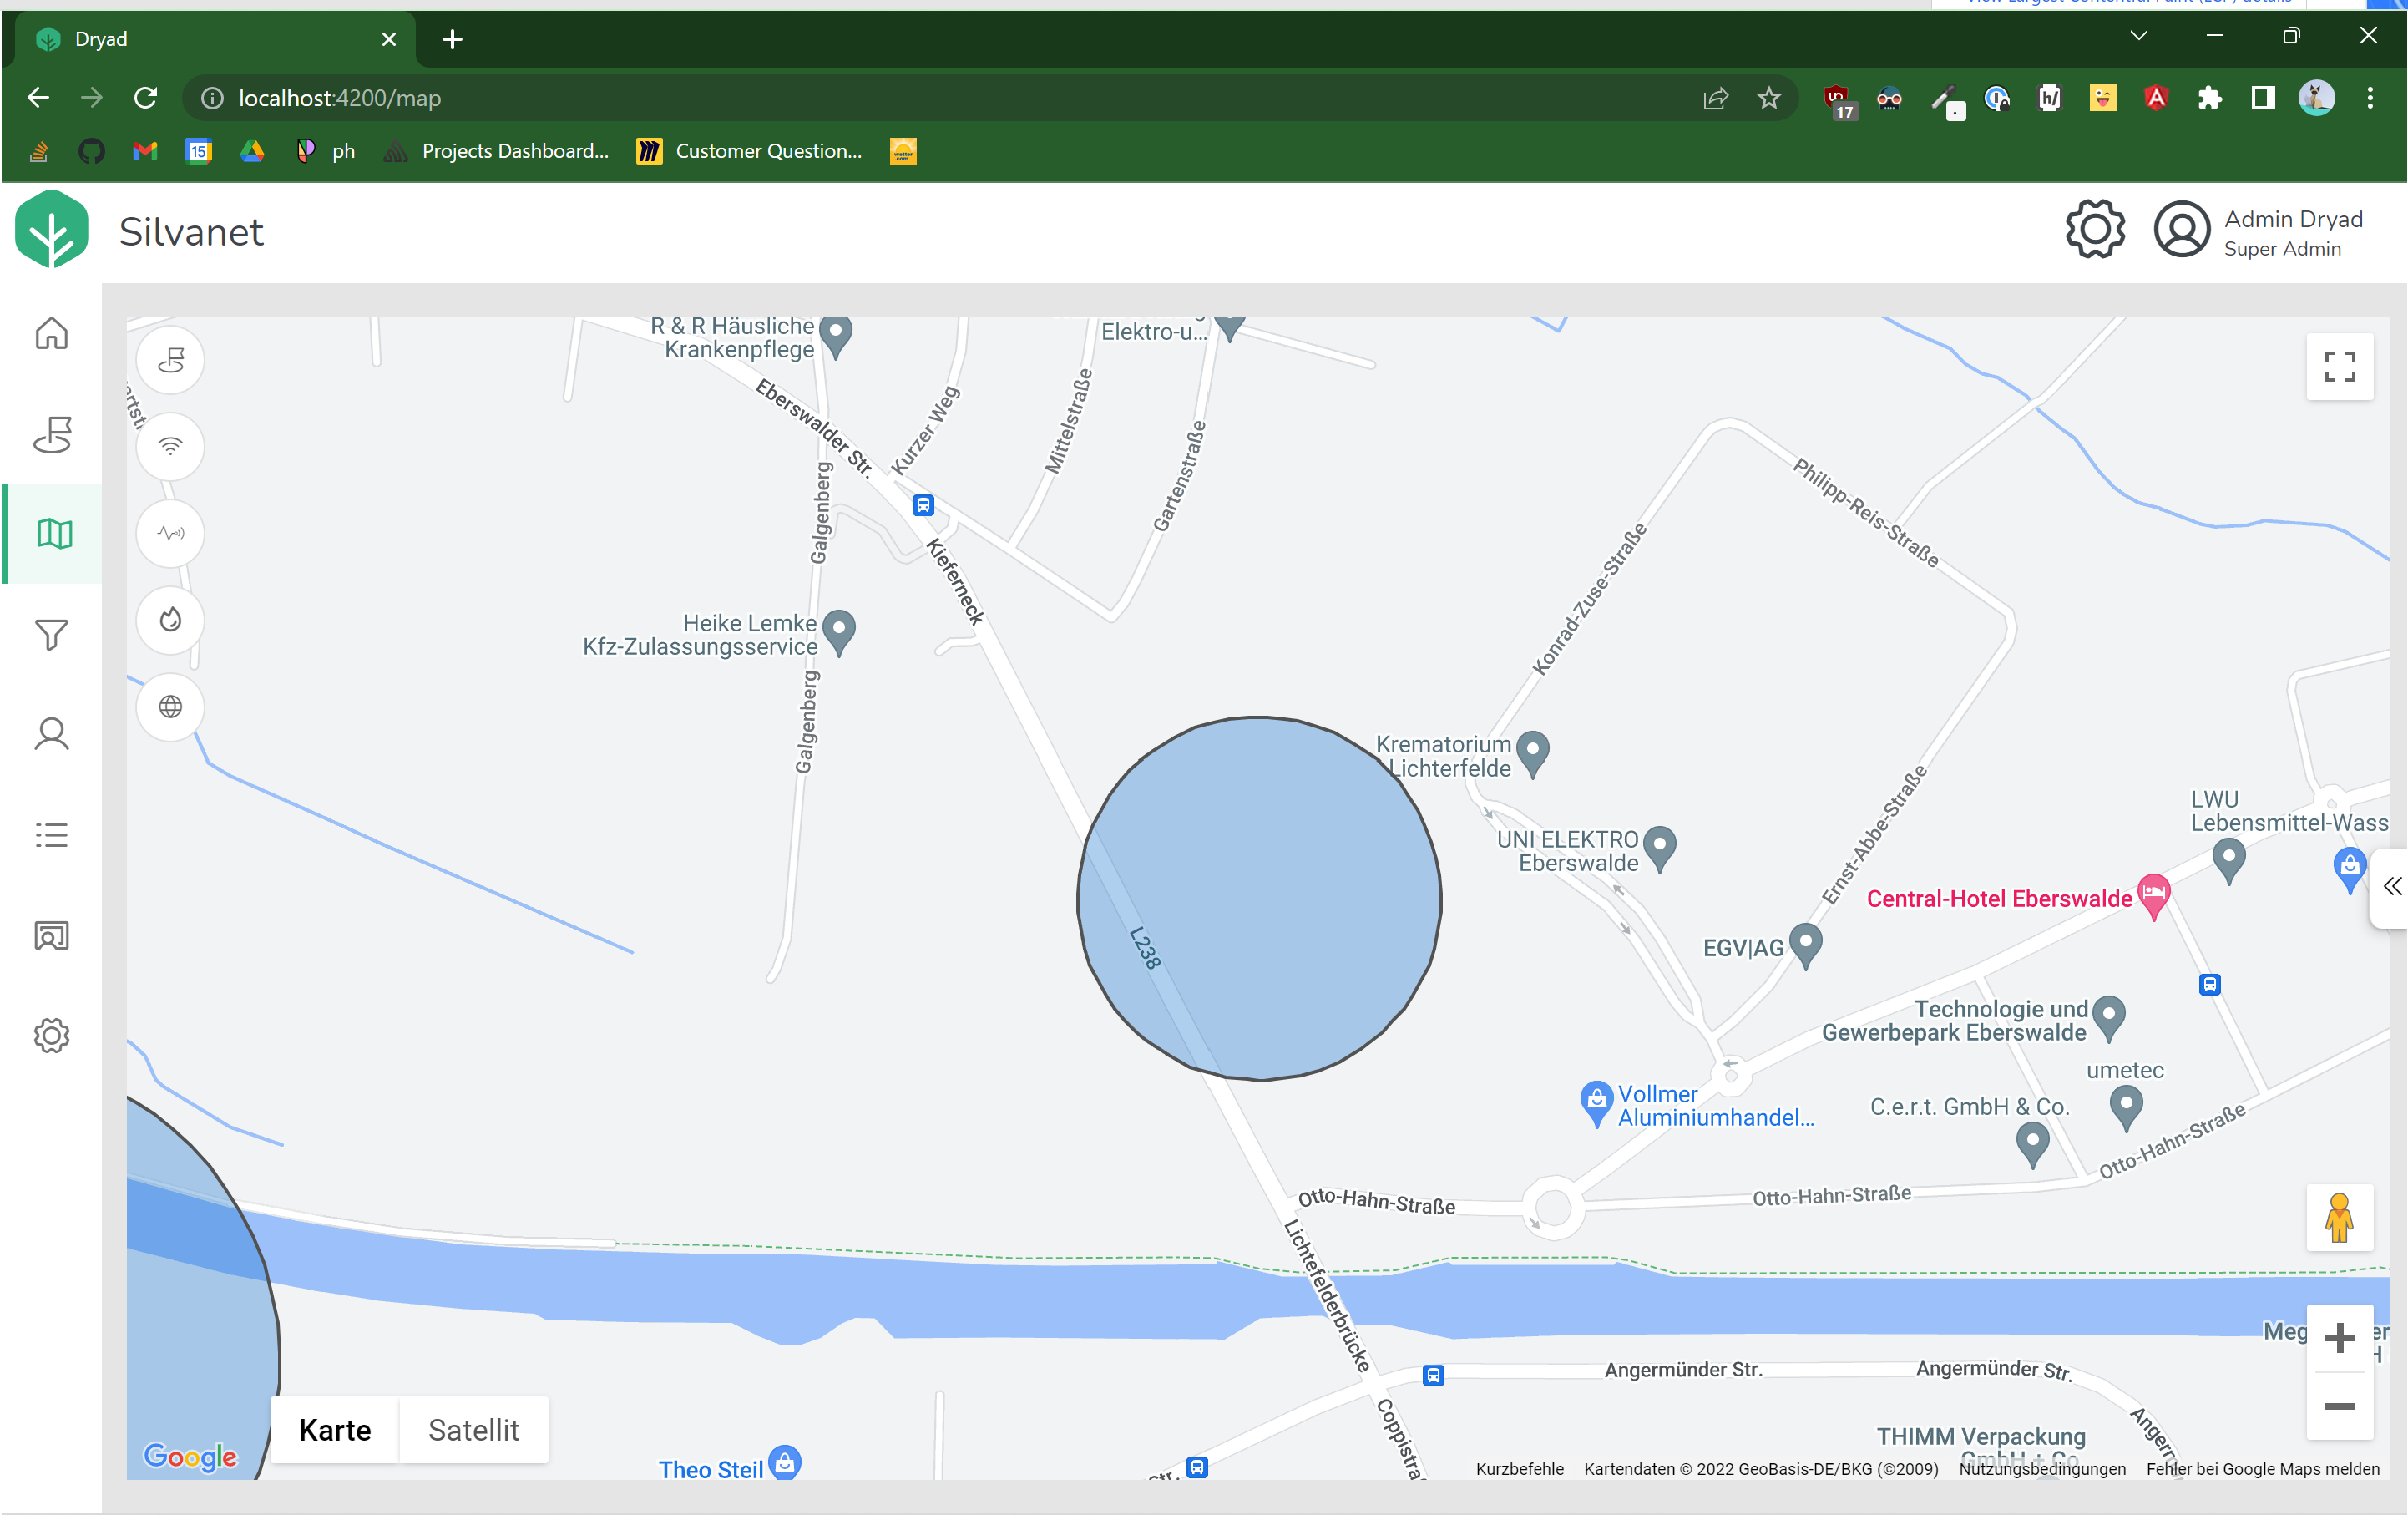
\includegraphics[width=\textwidth]{app_page_map_old}
  \caption{Seite der Schnittstelle mit einer interaktiven Karte der verschiedenen \textit{Sites}}
  \label{fig:app_page_map_old}
\end{figure}
\begin{figure}[H]
  \centering
  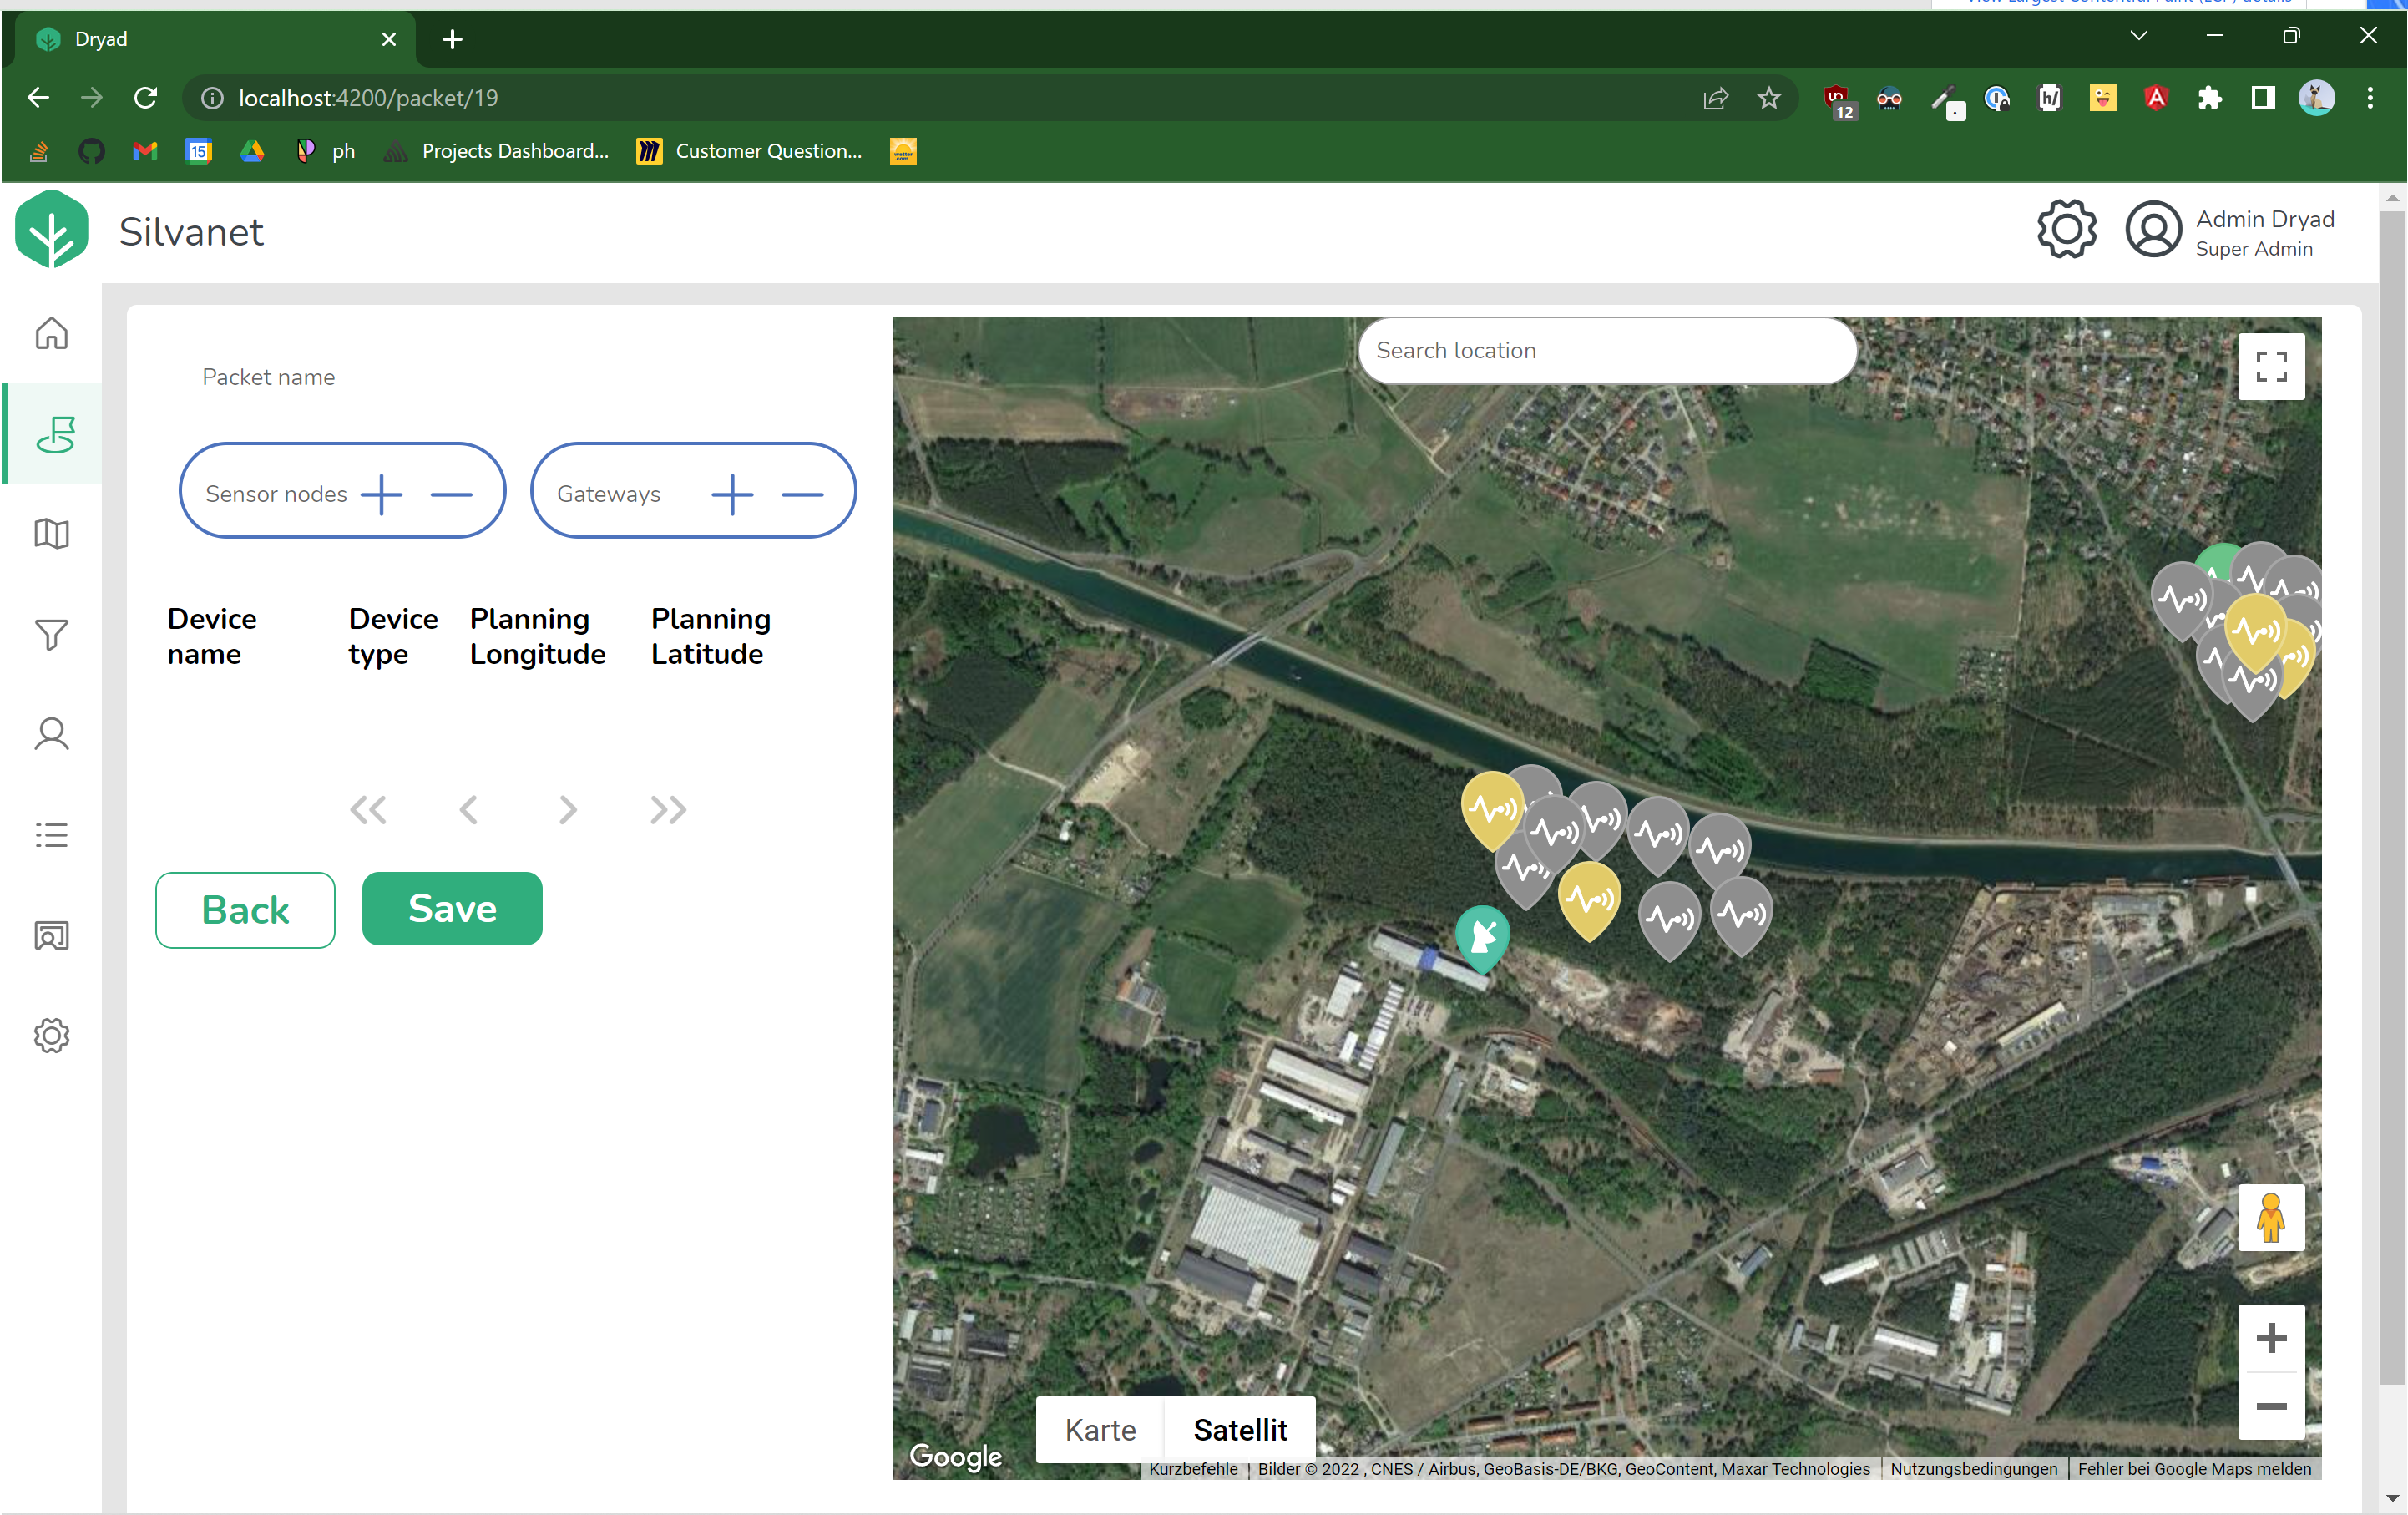
\includegraphics[width=\textwidth]{app_page_planning_old}
  \caption{Seite der Schnittstelle, mit der Sie den Einsatz von Sensoren an einem \textit{Sites} planen können.}
  \label{fig:app_page_planning_old}
\end{figure}

Auf diese Weise ist es für einen Nutzer nicht möglich, zu definieren, auf welcher Seite er sich befindet.
Es gibt jedoch viele standardisierte Strategien, die ein entspanntes Surfen ermöglichen.
Die erste, die sogar ein Muss für die Zugänglichkeit einer Schnittstelle ist, ist das Vorhandensein eines aussagekräftigen Seitentitels.
Dieser Seitentitel wird in \ac{HTML} im Header der Seitenstruktur deklariert und ermöglicht es, einen benutzerdefinierten String in der Titelleiste des Browsers, im Seitenfenster oder auch im Verlauf des Browsers anzuzeigen.
Anhand eines aussagekräftigen Titels kann ein Benutzer leicht erkennen, welche Webseite er gerade benutzt und wann sich die Webseite geändert hat.
Der Titel kann zur Identifizierung der Webseite verwendet werden, ohne dass die Benutzer den Inhalt der Seite lesen oder interpretieren müssen.
Die Benutzer können den gewünschten Inhalt schneller finden, wenn genaue, beschreibende Titel in Sitemaps oder Listen von Suchergebnissen erscheinen.

So empfehlen die Zugänglichkeitsstandards der \ac{WCAG}\cite{wcag}, dass der Titel einer Seite in der Lage ist:

\begin{itemize}
  \item Das Thema der Webseite identifizieren
  \item Sinn machen, wenn sie ohne Kontext gelesen werden, z. B. in einer Website-Karte oder einer Liste von Suchergebnissen
  \item Kurz sein
  \item Angabe der Website oder einer anderen Ressource, zu der die Webseite gehört
\end{itemize}

Eine Struktur, die von der großen Mehrheit der Web-Schnittstellen verwendet wird, kann durch die folgende Notation dargestellt werden\\
\lstinline{<Eindeutiger Titel der Seite> <Trenner> <Titel der Anwendung>}.

Im Fall der Silvanet-Anwendung von Dryad wurden die folgenden Standards festgelegt:

\begin{itemize}
  \item \textbf{<Titel der Anwendung>}: Dryad
  \item \textbf{<Trenner>}: •
\end{itemize}

Die Anwendung muss also in der Lage sein, für jede Seite einen Titel vorzuschlagen, der diesem Standard entspricht.
Jetzt müssen Sie dem Nutzer auch noch einen Seitentitel anbieten, der für die Seite selbst relevant ist.
Wie man in \ref{fig:app_page_map_old} und \ref{fig:app_page_planning_old} sehen kann, bleibt der Haupttitel der Seite, der dem \lstinline{h1}-Tag in \ac{HTML} entspricht, nämlich konstant das gleiche Wort \textit{Silvanet}.

Die Schnittstelle sollte an dieser Stelle auch einen Begriff verwenden, der den Kontext der Seite beschreibt, so dass er den Seitentitel widerspiegelt.
Hier ist ein Beispiel für eine Kombination von Seitentiteln mit einem relevanten, standardisierten und kontextbezogenen Hauptseitentitel.

\begin{table}[H]
  \begin{tabular}{p{0.5\linewidth} |p{0.5\linewidth}}
    Seitentiteln                   & Hauptseitentitel \\ \hline\hline

    \textit{Sites • Dryad}         & Sites Management \\\hline
    \textit{User Settings • Dryad} & User Settings    \\\hline
    \textit{Dashboard • Dryad}     & Dashboard
    \\\hline
  \end{tabular}
  \caption{Beispiel für eine Kombination von Seitentiteln mit einem Hauptseitentitel}
\end{table}

\subsection{Übersichtliches Navigationssystem}

Die Navigation des Nutzers sollte so einfach wie möglich gestaltet werden, damit es keine Ambiguität gibt, die es dem Nutzer erlaubt, die Oberfläche selbst zu erkunden.
Die ergonomische Inspektion \ref{appendix:ergonomic-inspection} zeigt jedoch einen großen Usability-Fehler in der Seitenleiste der Anwendung, die als Navigationsmenü fungiert.
Es besteht nur aus Icons, die, wie im Punkt \ref{sec:guidance} erläutert, sehr subjektiv und hängen von der Kultur des Nutzers ab.
Es ist daher notwendig, jedem Icon ein Textlabel hinzuzufügen, um die Verständlichkeit der Icons im Menü zu standardisieren.
Dies nimmt jedoch Platz auf der Benutzeroberfläche in Anspruch, da der Benutzer diese Aktion schnell beherrschen und verstehen muss.
Nach mehreren Besuchen auf der Benutzeroberfläche wird der Benutzer natürlich eine Verbindung zwischen den Icons und dem Label herstellen.
So ist es sinnvoll, dass der Nutzer jederzeit entscheiden kann, ob er die Textkennzeichnungen ausblenden oder anzeigen möchte.
In dieser Situation kann ein Kollaps-System verwendet werden.

\begin{table}[H]
  \begin{tabular}{p{0.5\linewidth} |p{0.5\linewidth}}
    Menü mit Textlabels & Reduziertes Menü nur mit Icons \\ \hline\hline

    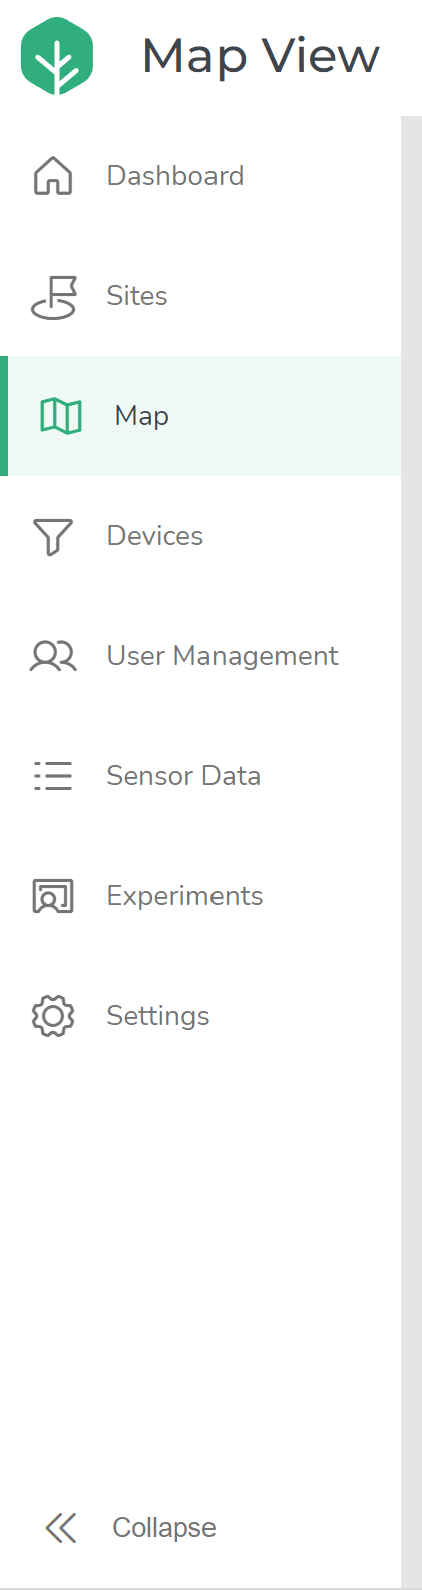
\includegraphics[height=12cm]{app_sidebar_open}
                        &
    
\includegraphics[height=12cm]{app_sidebar_collapsed}
  \end{tabular}
  \caption{Menü in der Sidebar, das ein Kollaps-Design implementiert}
\end{table}

\section{Gezielte ergonomische Verbesserungen} \label{sec:analyse-ergo}

Die Kriterien von Bastien und Scapin haben sehr gezielte Lücken in der Benutzeroberfläche aufgedeckt.
Die Benutzertests zeigten verwirrendes Verhalten, das auf einen Mangel an intuitiver Usability hindeutet.
Dieser Teil konzentriert sich daher auf die Behebung von Mängeln im Zusammenhang mit der Fehlerbehandlung, die Anpassung der Benutzeroberfläche und die Einführung von UI-Konzepten, die eine einfache Entdeckung einer neuen Benutzeroberfläche ermöglichen.

\subsection{Intuitive Verwaltung und Design von Fehlern}

Es ist wichtig zu verstehen, dass \ac{UX} und \ac{UI} Hand in Hand gehen; man kann das eine nicht ohne das andere haben.
Wie Rahul Varshney so treffend zitiert hat: ``UX ohne UI ist wie der Rahmen einer Skulptur ohne Pappmaché darauf. Ein großartiges Produkterlebnis beginnt mit UX, gefolgt von UI. Beide sind für den Erfolg des Produkts unerlässlich.''.
Daher scheint es sinnvoll zu sein, dem Nutzer die freundlichste aller möglichen UIs anzubieten.
Aus Zeitgründen sollte man sich auf die Teile der Anwendung konzentrieren, die am meisten davon profitieren.
Dies gilt insbesondere für Seiten, auf denen sich der Nutzer verletzlich und gestresst fühlt. Ein gutes Beispiel sind Fehlerseiten.
Dies lässt sich damit begründen, dass Nutzer eine positive emotionale Reaktion auf visuelles Design haben, was sie toleranter gegenüber kleineren Problemen mit der Benutzerfreundlichkeit Ihrer Website macht \cite{aestheticEffect}.
Daher neigen Menschen dazu zu glauben, dass Dinge, die besser aussehen, auch besser funktionieren - auch wenn sie nicht wirklich effektiver oder effizienter sind.
Dieses Phänomen heißt \textit{Der Ästhetik-Nutzungs-Effekt}.

\subsubsection{Darstellung des Fehlers}

Ein Beispiel für eine in der Webwelt recht verbreitete Fehlerrückmeldung ist eine 404-Seite, die anzeigt, dass die vom Benutzer angeforderte Ressource nicht oder nicht mehr existiert.
Die Anwendung von Dryad hat eine solche dynamische Seite, die sich an die Art des Fehlers anpasst, enthält aber tiefe Mängel in Bezug auf \ac{UX} und \ac{UI}.

\begin{figure}[H]
  \centering
  
\includegraphics[width=\textwidth]{app_404_broken_error}
  \caption{Screenshot der Seite 404 der Schnittstelle}
  \label{fig:app_404_broken_error}
\end{figure}

Das Design ist völlig kaputt und es gibt keine Aktionen für den Benutzer, was zu einer schlechten Erfahrung führt.
Auch gibt es hier keine UI-Elemente, die die Ästhetik der Seite unterstützen sollen.
Um diese Art von Fehlerseite interessanter zu gestalten, wäre es sinnvoll, eine kleine animierte Illustration und eine Fallback-Aktion einzufügen, die dem Nutzer die Orientierung erleichtert.
Auch die Beschreibung des Fehlers könnte sympathischer gestaltet werden, indem man mit der Sensibilität des Nutzers spielt.
So könnte man sich für die Beschreibung einer 404-Seite vorstellen, "Die von Ihnen angeforderte Seite kann nicht gefunden werden" durch "Die von Ihnen gesuchte Seite kann umbenannt, gelöscht oder nie auf der Erde existieren" zu ersetzen.

Für die Illustrationen ist es sinnvoll, die bereits von Dryad erstellten Grafiken und Farben beizubehalten.
Die folgenden Illustrationen wurden mit dem Figma-Tool erstellt und werden jeweils von links nach rechts für eine nicht existierende Seite, den Zugriff auf eine Seite, die aufgrund fehlender Rechte verboten ist, und die Seite, die anzeigt, dass eine angeforderte Ressource nicht existiert, verwendet.
Sie wurden im \ac{SVG}-Format erstellt, sodass sie wie das \ac{DOM} einer Webseite manipuliert werden können, sodass sie einfach mit der \ac{CSS}-Sprache animiert werden können und auch beliebig skalierbar sind, da es sich um Vektorbilder handelt.

\begin{figure}[H]
  \centering
  
\includegraphics[width=\textwidth]{errors_illustation}
  \caption{Illustrion verwendet mit verschiedenen Fehlermeldungen der Schnittstelle}
  \label{fig:errors_illustation}
\end{figure}

Die Anwendung sollte daher in der Lage sein, relevantere und sympathischere Fehlerseiten wie folgt anzuzeigen:

\begin{figure}[H]
  \centering
  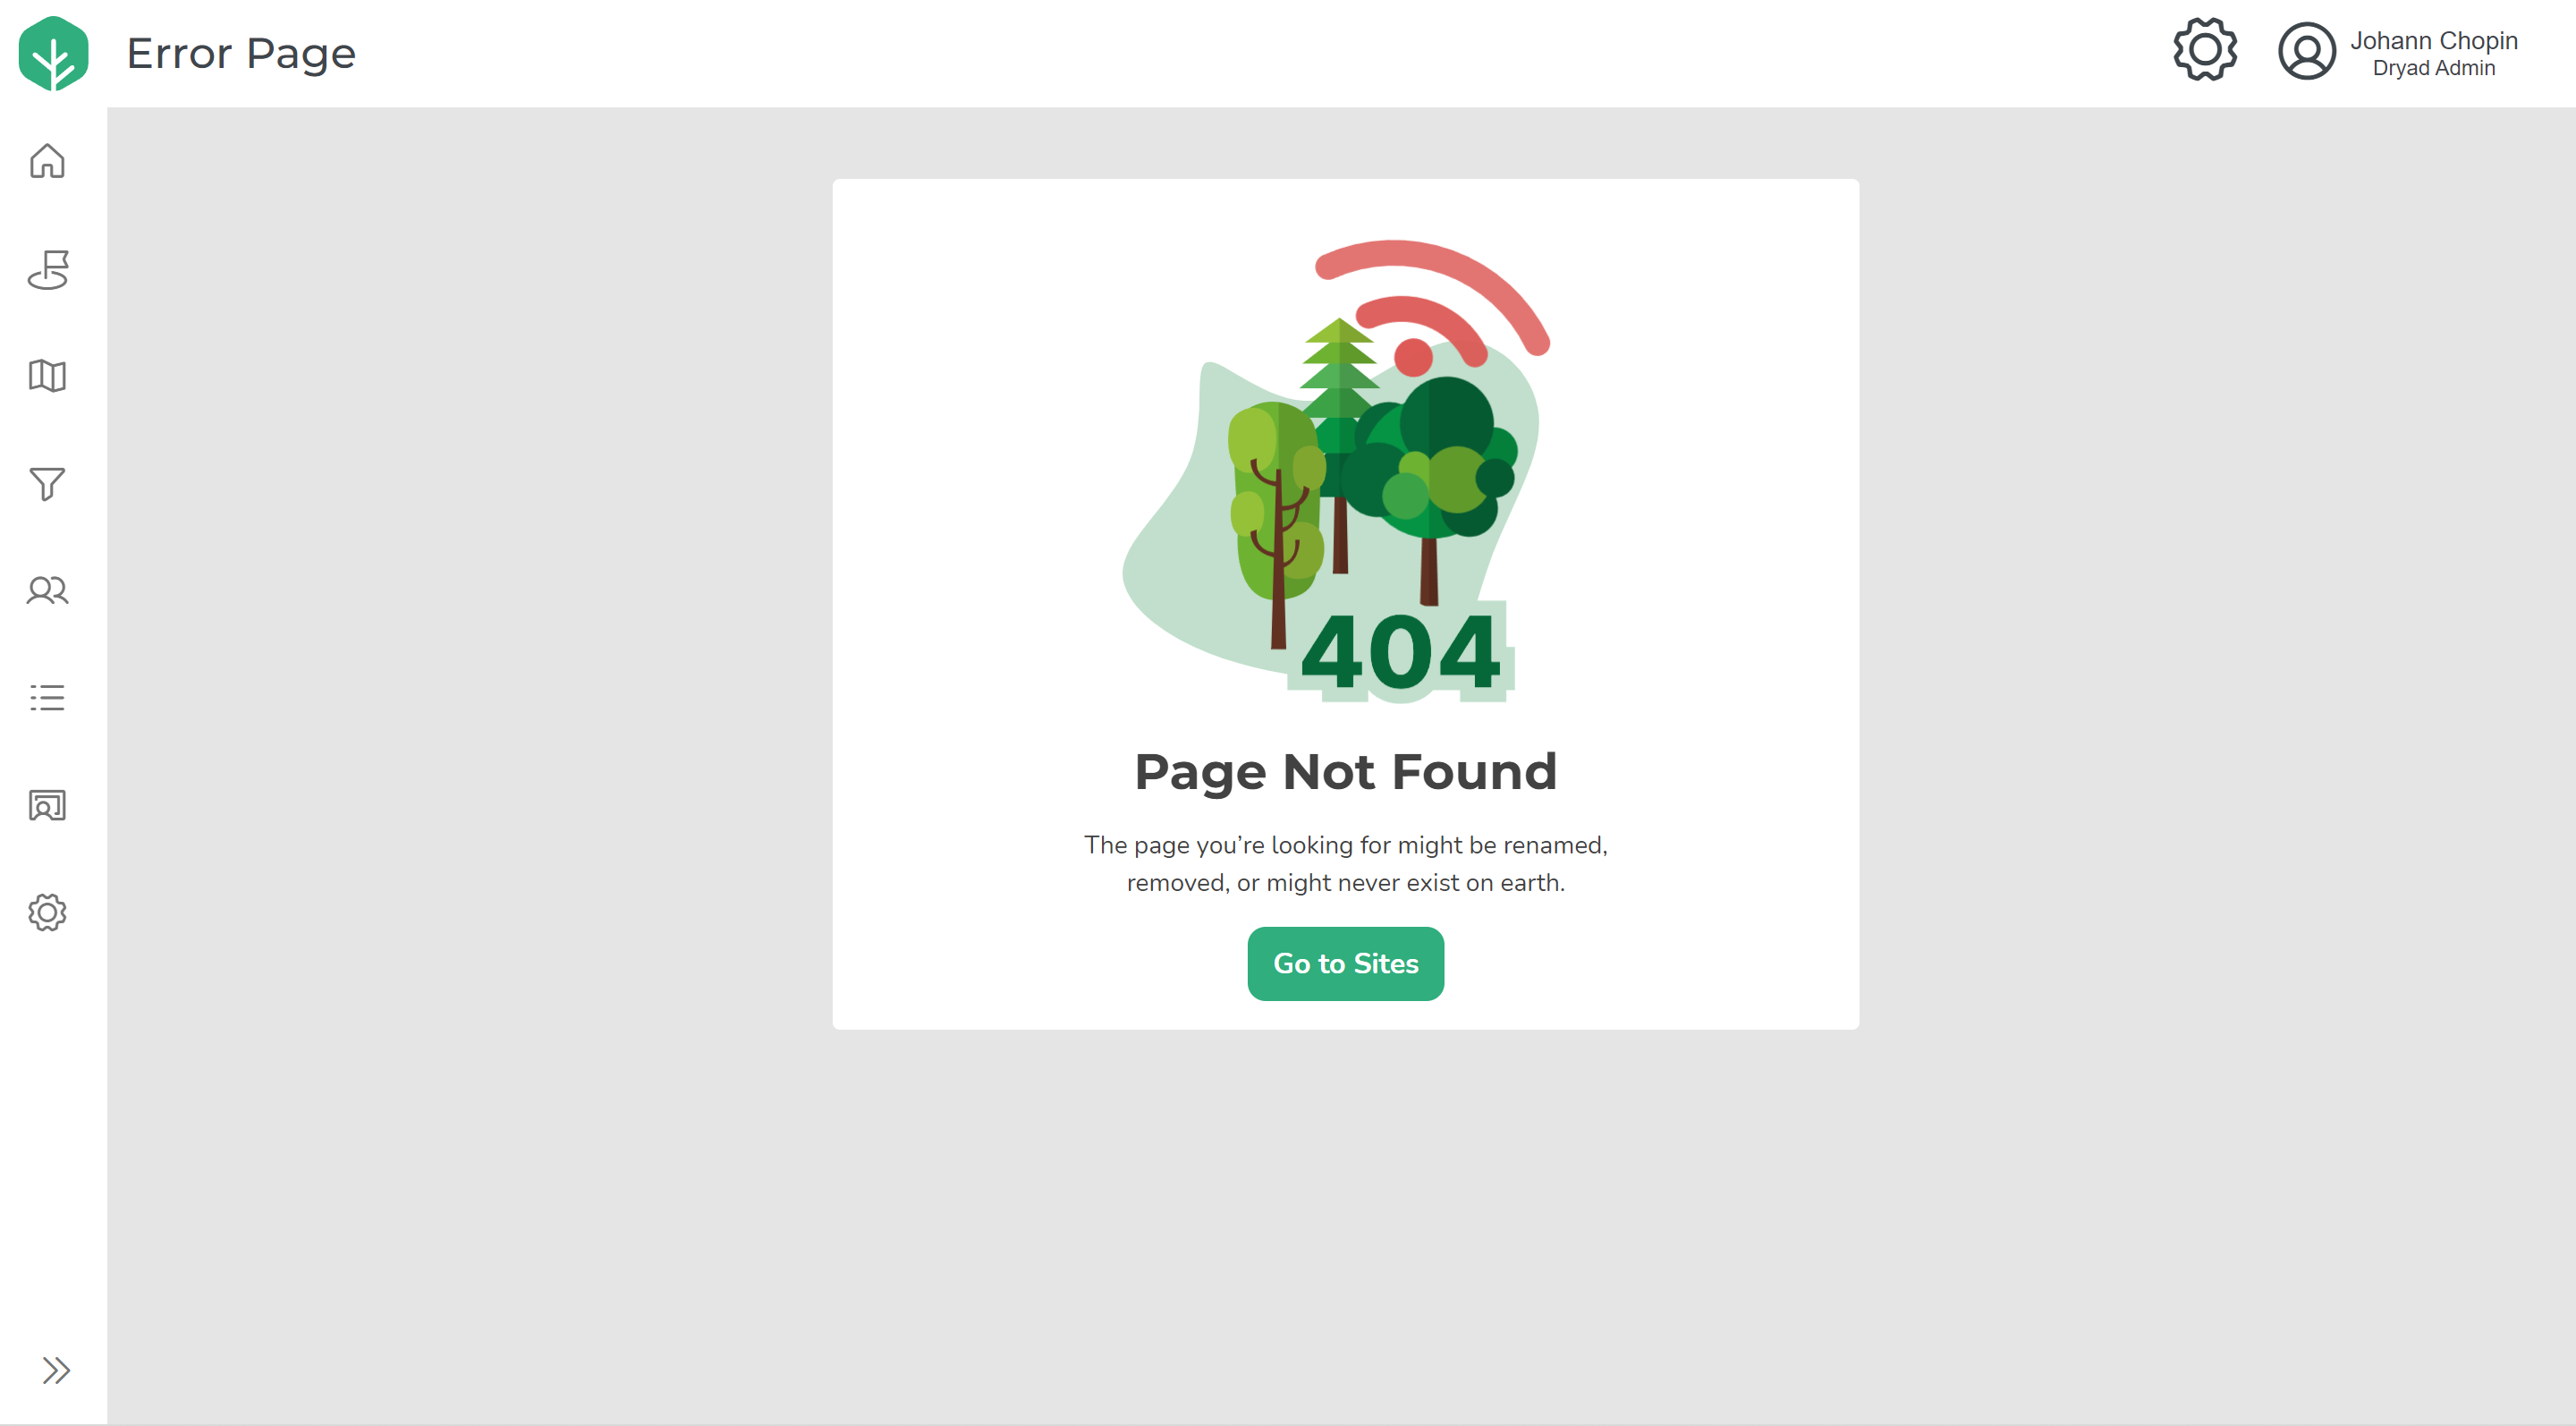
\includegraphics[width=13cm]{app_404_new}
  \caption{Prototyp der neuen 404-Seite}
  \label{fig:app_404_new}
\end{figure}

\begin{figure}[H]
  \centering
  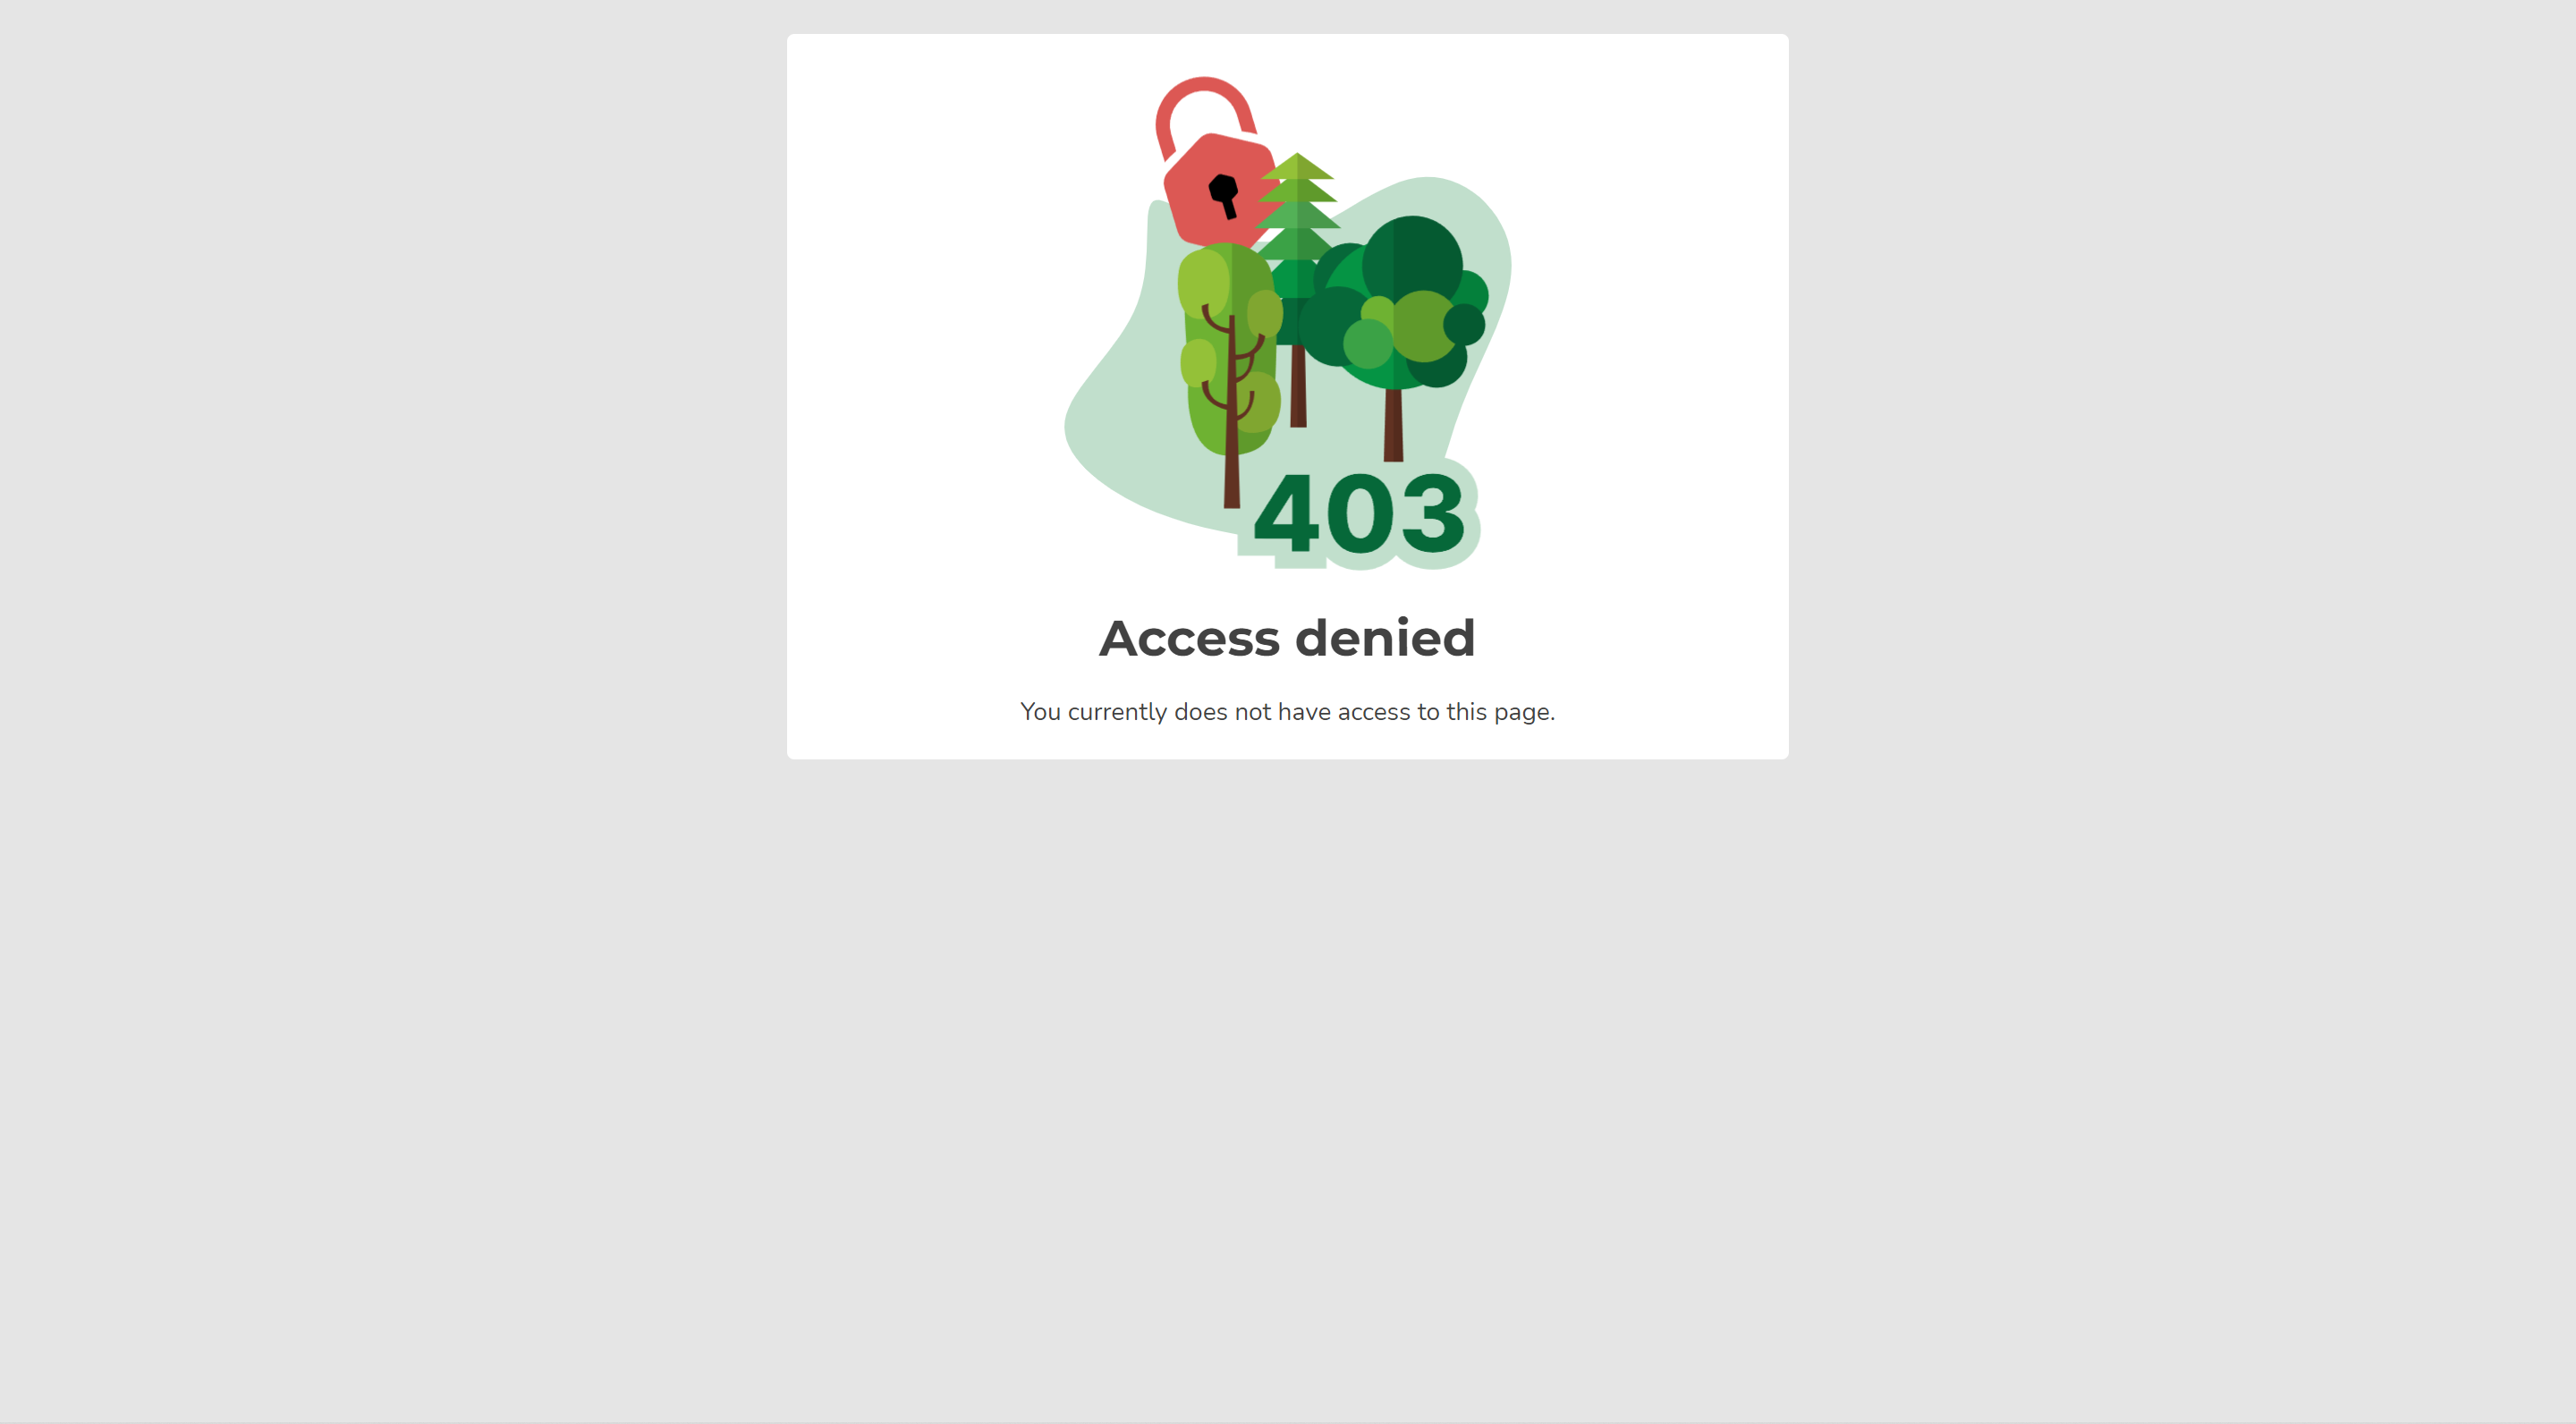
\includegraphics[width=13cm]{app_403}
  \caption{Prototyp der Seite, die einem Benutzer angezeigt wird, der versucht, ohne die erforderlichen Rechte auf eine Seite zuzugreifen.}
  \label{fig:app_403}
\end{figure}

\subsubsection{Darstellung der Stabilität}

Dieses UI-Design mit Illustrationen kann auch für andere Zwecke als die Anzeige von Fehlern verwendet werden.
Ein gutes Beispiel und die Alert-Seite, die von slug \lstinline{/alert-centre} aus verfügbar ist.
Wenn keine Warnmeldungen erkannt werden, ist die Seite einfach nur leer.
Wenn Sie in diesem Fall eine animierte Abbildung eines friedlichen Waldes mit den verschiedenen Sensoren des Silvanet-Systems hinzufügen, wird der Benutzer, wenn er sie sieht, beruhigt und die verfügbaren Produkte werden noch einmal hervorgehoben.

\begin{figure}[H]
  \centering
  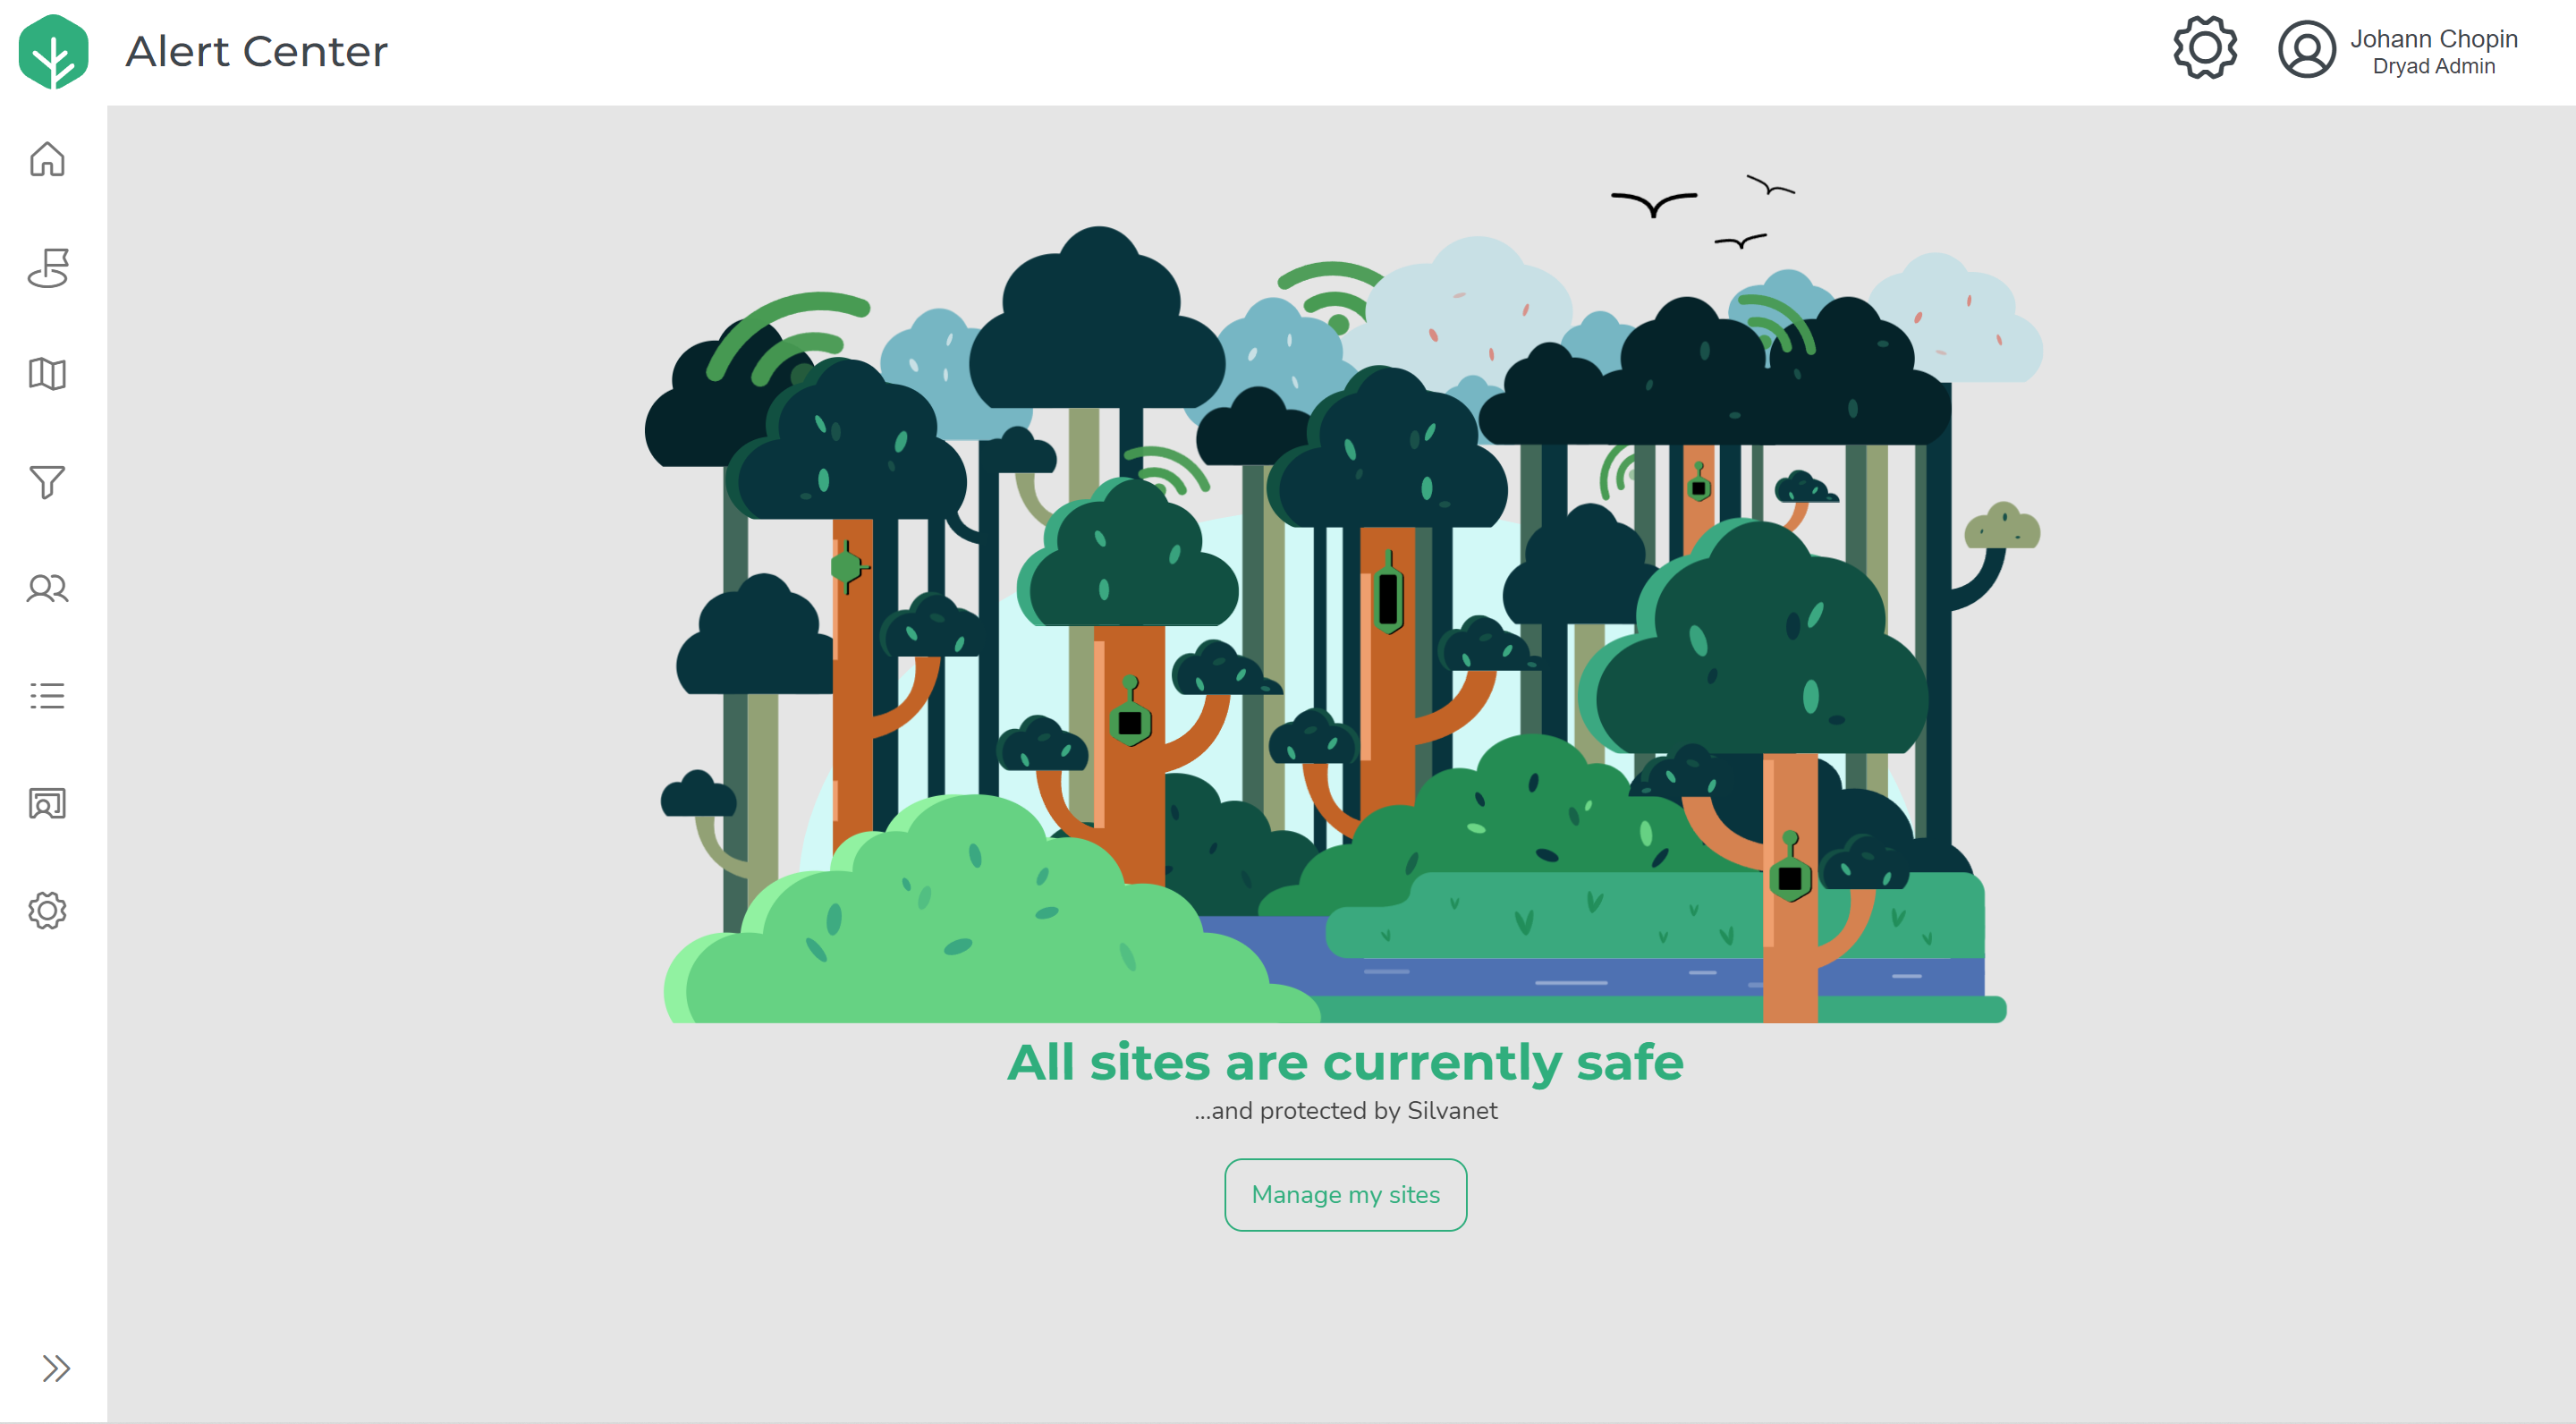
\includegraphics[width=\textwidth]{app_alert_center_safe}
  \caption{Seite des Alert-Centers, auf der angezeigt wird, dass derzeit keine Alerts detektiert werden}
  \label{fig:app_alert_center_safe}
\end{figure}

\subsubsection{Mechanismus zur Alarmierung bei Feuererkennung}

Wenn das Silvanet-System einen Waldbrandalarm erkennt, wird eine E-Mail an alle Personen gesendet, die als Verantwortliche für den betreffenden \textit{Site} aufgelistet sind.
Auf der Webschnittstelle kann man sich über ein Echtzeitsystem auch anzeigen lassen, wenn eine Alarmierung erkannt wurde.
Sie ist mit einem Websocket-Kanal verbunden, der es ermöglicht, in Echtzeit verschiedene Informationen zu empfangen und zu versenden, insbesondere Warnungen vor Waldbränden.
Wenn ein Alert auftritt, blinkt derzeit im Header der Seite ein Link, der zur Seite des Alert Centers weiterleitet (siehe \ref{fig:app_fire_alert_button_badge}).
Benutzertests haben gezeigt, dass die Anzeige der Anzahl der Alarme (entsprechend der Anzahl der Sensoren, die Rauch erkennen) für den Benutzer verwirrend war, da er nicht wusste, was er von dieser Zahl halten sollte.
Außerdem führt das rote Design des \ac{UI}-Elements und seine Blinkanimation dazu, dass der Nutzer sehr schnell und natürlich darauf klickt, ohne sich wirklich die Zeit zu nehmen, das Vorhandensein dieser Zahl zu identifizieren.
Da diese Nummer keinen Mehrwert bietet, überfrachtet sie die Benutzeroberfläche und kann daher entfernt werden. Außerdem sollte ein Flammen-Icon verwendet werden, um das Konzept des Feuers zu standardisieren.

\begin{figure}[H]
  \centering
  
\includegraphics[width=6cm]{app_fire_alert_button_v2}
  \caption{Prototyp der vereinfachten Schaltfläche zur Meldung einer Warnung}
  \label{fig:app_fire_alert_button_v2}
\end{figure}

Benutzertests zeigen, dass dieses \ac{UI}-Element sehr effektiv ist, um einen Alarm zu melden, wenn sich der Benutzer auf der Oberfläche befindet.
Leider ist diese Funktion nur dann nützlich, wenn sich der Benutzer auf der Anwendungsseite seines Browsers befindet.
Wenn der Nutzer eine andere Registerkarte seines Browsers besucht, ist er nicht in der Lage, höchstens eine Warnung zu erkennen.
Es ist jedoch möglich, die Aufmerksamkeit des Nutzers auf einen bestimmten Tab zu lenken, auch wenn er inmitten vieler anderer Tabs untergeht.
Jede Webseite wird in einem Tab durch ihren Titel und ein kleines Icon, das sogenannte \textit{Favicon}, symbolisiert.
Sie können dieses Favicon genauso blinken lassen wie die Schaltfläche, die zum Warnzentrum weiterleitet, indem Sie das Favicon standardmäßig mit demselben roten Favicon alarmieren, das die Gefahr anzeigt.
Das Gefahren-Favicon wird auch ein wenig von dem Standard-Favicon abweichen, so dass auch Menschen mit Problemen bei der Farberkennung eine Bewegung sehen können.

\begin{figure}[H]
  \centering
  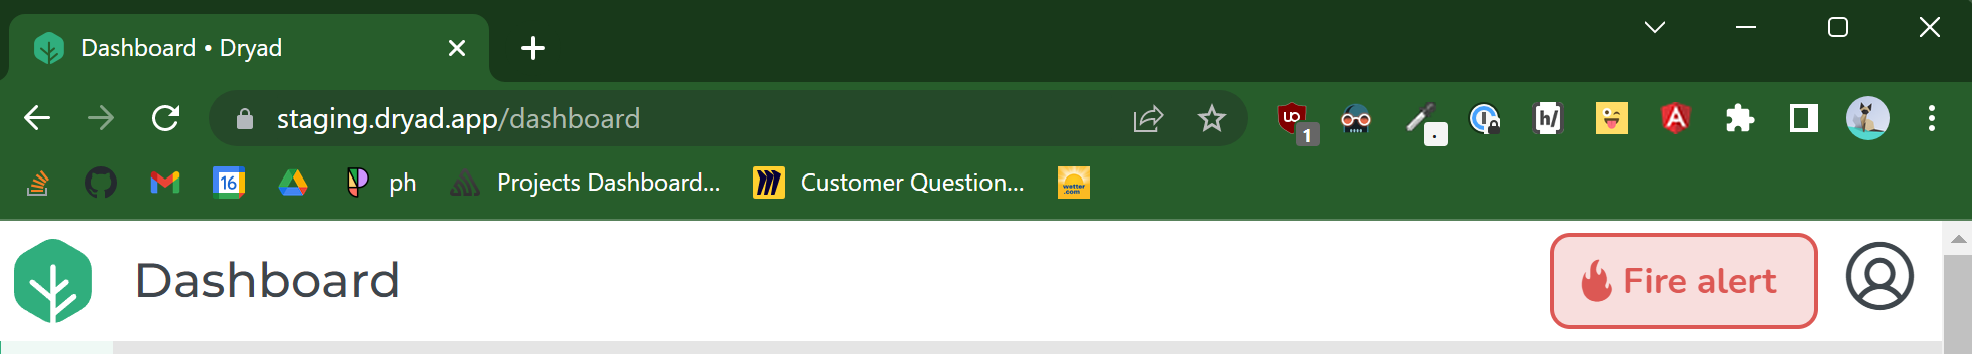
\includegraphics[width=\textwidth]{app_favicon_default}
  \caption{Standard-Favicon der Anwendung von Dryad (grünes Icon in der linken oberen Ecke)}
  \label{fig:app_favicon_default}
\end{figure}

\begin{figure}[H]
  \centering
  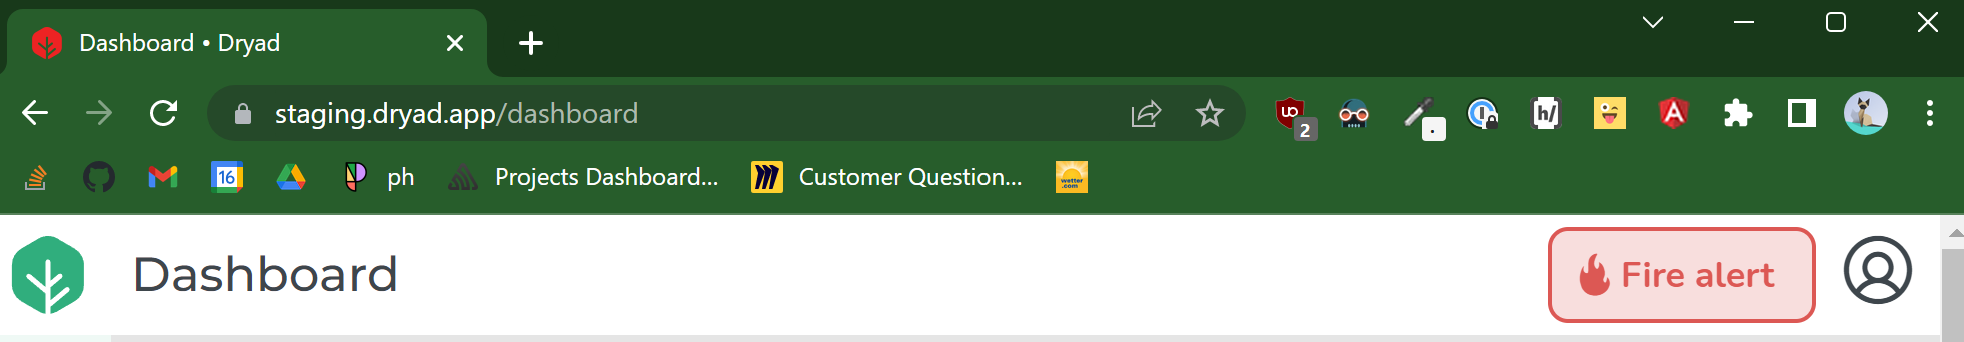
\includegraphics[width=\textwidth]{app_favicon_danger}
  \caption{Favicon der Dryad-App in einer roten Variante und leicht verschoben, um einen Tab mit einem Blinkeffekt hervorzuheben}
  \label{fig:app_favicon_danger}
\end{figure}

\subsection{Anwendungsanpassung und Lokalisierung} \label{sec:conceptionLocale}
Um dem Nutzer ein besseres Erlebnis zu bieten, ist es wichtig, dass sich die Benutzeroberfläche an den Nutzer anpasst und nicht umgekehrt.
Eine Anwendung sollte ein Werkzeug sein und nicht eine Einschränkung für den Nutzer.
Daher ist es sehr wichtig, dass sich die Schnittstelle automatisch anpasst oder angepasst werden kann, wo kulturelle Unterschiede auftreten.
Ein sehr auffälliges Beispiel ist die Anzeige von Entfernungsdaten, die nicht skaliert sind und ständig in metrischen Einheiten angezeigt werden.
So zeigt die Benutzeroberfläche immer wieder Daten wie die Fläche eines Geländes von 225300 Quadratmetern an, was dem Benutzer viel Mühe bereitet, sich diese Größe vorzustellen, während 22,53 Hektar viel leichter verdaulich sind.
Außerdem ist die Schnittstelle auch für den amerikanischen Markt bestimmt, der das Imperialsystem mit Einheiten wie Fuß, Meile oder Acre für Flächen verwendet.

In der gleichen Idee sollte es möglich sein, auszuwählen, wie das Datums- und Zeitformat angezeigt werden soll.
Die verschiedenen Optionen werden zwischen dem metrischen und dem imperialen System unterschieden.

\begin{table}[H]
  \centering
  \begin{tabular}{l c c}
    \toprule % Top horizontal line
                             & \multicolumn{2}{c}{\textbf{Messsystem}}                               \\
    \cmidrule(l){2-3}
    \textbf{Datentyp}        & Metrisches System                       & Imperialsystem              \\
    \midrule % In-table horizontal line
    Entfernungen und Flächen & m, km, und ha                           & ft, mile und acre           \\
    Datum                    & dd/mm/yyyy                              & yyyy-mm-dd                  \\
    Uhrzeit                  & 24-Stunden-Format (22:00)               & 12-Stunden-Format (10:00PM) \\
  \end{tabular}
  \caption{Einheitenformat, das auf dem metrischen oder imperialen System basiert}
\end{table}

Die Benutzeroberfläche sollte in der Lage sein, automatisch zu erkennen, welches Messsystem verwendet wird.
In einem zweiten Schritt sollte der Benutzer eine Seite mit Präferenzen erhalten, auf der er auswählen kann, welche Formate er für die verschiedenen Datentypen verwenden möchte.
Die automatische Erkennung erfolgt durch die Erkennung der Sprache des Browsers des Nutzers.
Wenn die Standardsprache amerikanisches Englisch oder British English ist, das in RFC5646 \cite{rfc5646} als \textit{en-US} und \textit{en-GB} bezeichnet wird, dann wird das imperiale System verwendet.
Im umgekehrten Fall wird das metrische System verwendet.

Die Konvertierung zwischen den verschiedenen Größenordnungen von Entfernungen und Flächen sollte automatisch von der Schnittstelle vorgenommen werden, um dem Nutzer die relevanteste Darstellung zu bieten.
Dies ist recht einfach zu bewerkstelligen, da alle Daten in Metern für die Entfernungen und in Quadratmetern für die Einheiten angegeben sind.
Die verschiedenen Größenordnungen und ihre jeweiligen Einheiten in Abhängigkeit vom verwendeten System sind in den folgenden Tabellen aufgelistet.

\begin{table}[H]
  \centering
  \begin{tabular}{l c c}
    \toprule
                                  & \multicolumn{2}{c}{\textbf{verwendete Einheit}}                  \\
    \cmidrule(l){2-3}
    \textbf{Entfernung in Metern} & Metrisches System                               & Imperialsystem \\
    \midrule
    < 1000 Metern                 & Meter (m)                                       & Fuß (ft)       \\
    >= 1000 Metern                & Kilometer (km)                                  & Meilen (mile)  \\
  \end{tabular}
  \caption{Einheit, die je nach Größenordnung der Entfernung verwendet wird}
  \label{table:metric_order_magnitude}
\end{table}

\begin{table}[H]
  \centering
  \begin{tabular}{l c c}
    \toprule
                                    & \multicolumn{2}{c}{\textbf{verwendete Einheit}}                      \\
    \cmidrule(l){2-3}
    \textbf{Fläche in Quadratmeter} & Metrisches System                               & Imperialsystem     \\
    \midrule
    < 10.000 Quadratmetern          & Quadratmeter (m²)                               & Quadratfuß (ft²)   \\
    >= 10.000 Quadratmetern         & Hektar (ha)                                     & Acre (acre)        \\
    >= 1.000.000 Quadratmetern      & Quadratkilometer (km²)                          & Quadratmeile (mi²) \\
  \end{tabular}
  \caption{Einheit, die je nach Größenordnung der Fläche verwendet wird}
\end{table}

\subsection{Design mit kognitivem Tunnelsystem}

Die Tatsache, dass ein Benutzerhandbuch eingeführt wird, das dem Benutzer erklärt, wie die Schnittstelle bedient wird, weist direkt auf Lücken in der entdeckenden Usability hin.
Die Benutzertests bestätigten dies, indem sie insbesondere eine gewisse Hesitation bei der Nutzung der Seite zeigten, auf der man den Einsatz von Sensoren für einen bestimmten \textit{Site} planen kann.
Darüber hinaus präsentiert diese Schnittstelle dem Nutzer eine Informationsbox, die Punkt für Punkt erklärt, wie sie zu verwenden ist.
Dies ist zwar eine gute Strategie, um den Nutzer zu führen, deutet aber dennoch auf einen Mangel an intuitiver Nutzbarkeit hin.
Es ist möglich, im Anhang \ref{appendix:planing_devices_flow} den Track des Benutzers einzusehen, um einen Sensor hinzuzufügen, der an einem \textit{Site} mit bestimmten Koordinaten eingesetzt werden soll.
Das Verhalten der Anwendung in Bezug auf die verschiedenen Kernbereiche der UI kann mit dem folgenden Zustandsdiagramm schematisch dargestellt werden.

\begin{figure}[H]
  \centering
  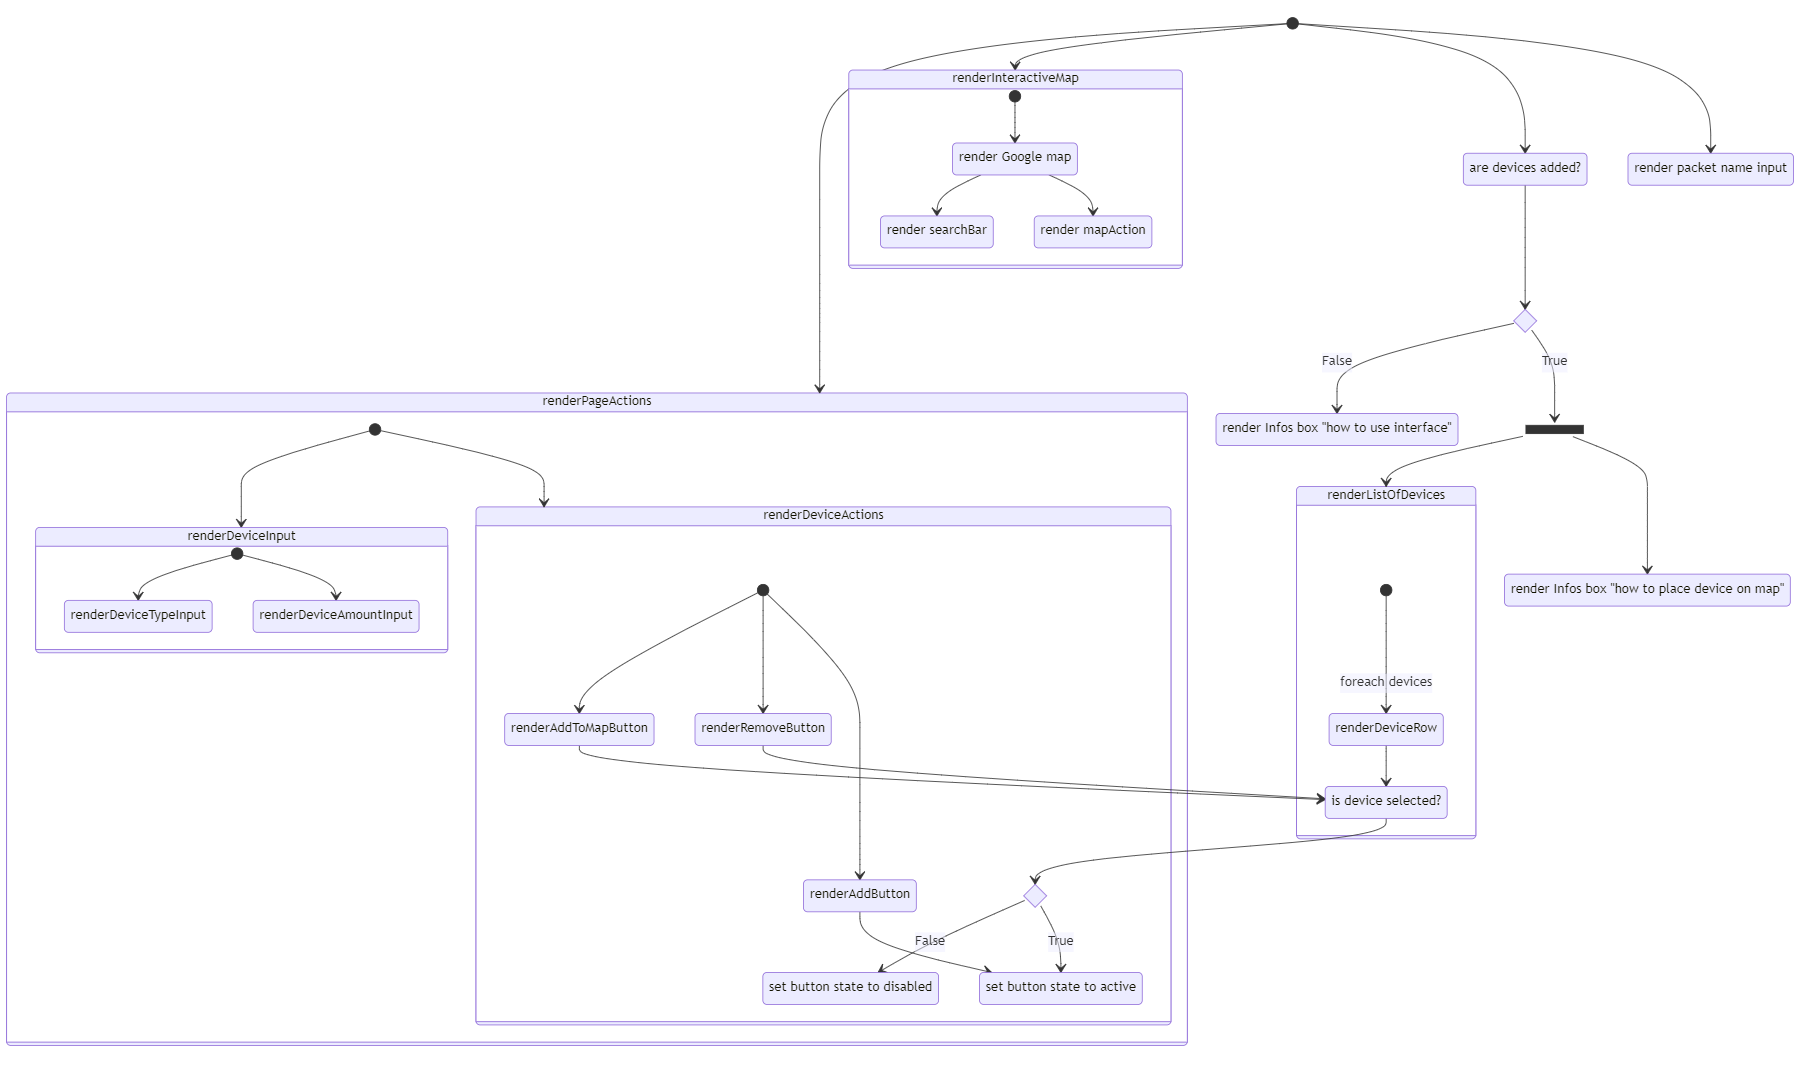
\includegraphics[width=17cm]{planing_v1_state_diagram}
  \caption{Zustandsdiagramm des Verhaltens der Schnittstelle zur Planung des Einsatzes einer \textit{Site} (Englisch)}
  \label{fig:planing_v1_state_diagram}
\end{figure}

Wenn man das Diagramm verfolgt und sich die Screenshots ansieht, wird schnell klar, dass sich der Benutzer sehr schnell mit einer Benutzeroberfläche konfrontiert sieht, die sehr viele Aktionsfelder hat, die nicht in Gruppen eingeteilt sind.
Ein auffälliges Beispiel sind die Schaltflächen \textit{Gerät aus der Liste entfernen} und \textit{Gerät aus der Liste auf der Karte platzieren}, obwohl es noch keine Einträge in der Liste gibt.
Diese beiden Schaltflächen überladen die Benutzeroberfläche unnötig mit Aktionen, die der Benutzer nur schwer verstehen kann, da er sich noch nicht bewusst ist, mit welchen Elementen sie interagieren.

Um dieses Problem einer zu komplexen und mit Handlungselementen beladenen Schnittstelle zu lösen, kann ein kognitives Tunnelsystem implementiert werden \cite{tunnelDesign}.
Tunnelling ist eine Strategie, die darauf abzielt, die Ablenkungen durch zusätzliche UI-Elemente zu beseitigen, um den Fokus des Benutzers auf ein einziges Ziel zu lenken.
Auf diese Weise fühlt sich der Nutzer, der sich in einem solchen Design wiederfindet, von der Benutzeroberfläche so geführt, dass er so wenig Fragen wie möglich stellen muss.
Ein konkretes Beispiel für diese Art von Design ist ein Step-by-Step-Formular für den Kauf eines Online-Artikels.
Zuerst werden Sie aufgefordert, die Bestellinformationen zu überprüfen, dann werden Sie nach der Lieferadresse gefragt, indem die vorherige Seite ausgeblendet wird, und schließlich werden Sie nach Ihren Kreditkarteninformationen gefragt, nachdem die vorherige Seite ausgeblendet wurde.
Im Fall der Planungsseite könnte man diese Informationsbox entfernen, indem man einfach die verfügbaren Aktionen nur dann anzeigt, wenn sie auch genutzt werden können.

Mit diesem Konzept ist es möglich, den Fluss der Seite auf das folgende Zustandsdiagramm zu reduzieren.
Ein visueller Prototyp, der diese Logik veranschaulicht, wurde ebenfalls entwickelt und kann in Anhang \ref{appendix:planing_devices_flow_tunneling} eingesehen werden.

\begin{figure}[H]
  \centering
  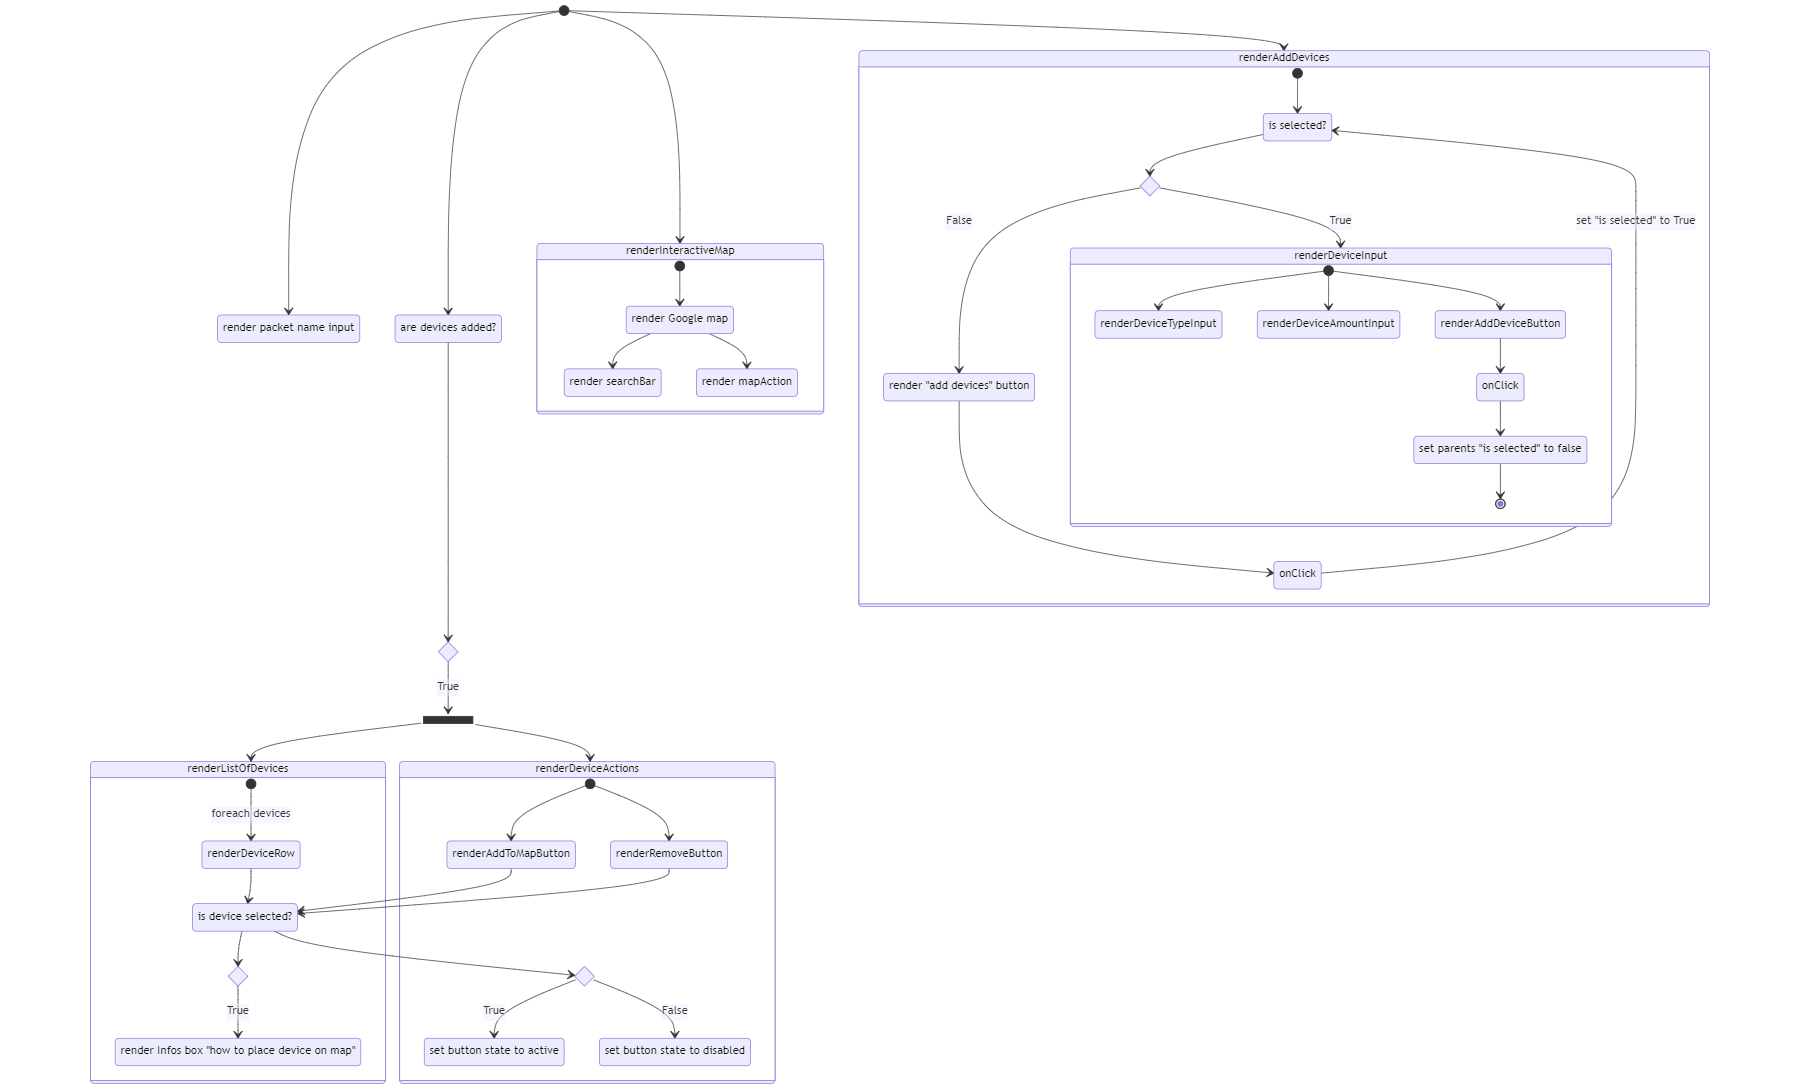
\includegraphics[width=17cm]{planing_v2_state_diagram}
  \caption{Zustandsdiagramm des Verhaltens der Schnittstelle \ref{fig:planing_v1_state_diagram}, die ein kognitives Tunnelsystem implementiert (Englisch)}
  \label{fig:planing_v2_state_diagram}
\end{figure}

Mit dieser Logik sieht der Benutzer eine leere Oberfläche, die nur die Aktionen anbietet, die er ausführen kann, wie z. B. das Paket über das Eingabefeld zu benennen oder ein Gerät über eine Drucktaste hinzuzufügen.
Wenn er auf die Schaltfläche klickt, dann erscheinen die verschiedenen Eingabefelder, mit denen er ein Gerät hinzufügen kann.
Sobald er die Geräte hinzugefügt oder abgebrochen hat, verschwinden die Eingabefelder und machen Platz für die Standardschaltfläche.
Das erhöht zwar die Anzahl der Aktionen, die notwendig sind, um zum Ziel zu gelangen, hat aber den Vorteil, dass die Benutzeroberfläche durch die Nutzung natürlich erlernt wird.

\section{Neudefinition des Verhaltens von interaktiven Karten} \label{sec:analyse-karten}

Die interaktiven Karten der App erwiesen sich in den Benutzertests als sehr enttäuschend und kaum nutzbar (siehe \ref{sec:user_tests_results}).
Es ist notwendig, neu zu überdenken, was die Nutzer von einer solchen Karte erwarten, um die für sie relevantesten Features anbieten zu können.
Dieser Teil wird sich auf die Ideation der zu implementierenden Features, die Darstellung der Gruppierung von Punkten in verschiedenen Clustern und die Auswahl der UI konzentrieren, die es ermöglicht, \textit{Sites} und ihre Sensoren mit ihrem jeweiligen Status geografisch zu repräsentieren.

\subsection{Ideation im Team}

Bei einer solch niedrigen Usability-Punktzahl ist es von entscheidender Bedeutung, die Ziele der interaktiven Karten, mit denen eine \textit{Site} angezeigt wird, neu zu bewerten.
Dazu wurde eine schnelle Brainstorming-Sitzung mit dem Cloud-Team durchgeführt.
Das Thema der Reflexion lautete: \textit{Was sollte auf der interaktiven Kartenseite möglich sein?}.
Der Fortschritt der Überlegungen zum Miro-Tool kann im Anhang \ref{appendix:question_board_map} nachgelesen werden, der sich in den folgenden Bedürfnissen zusammenfassen lässt:

\begin{table}[H]
  \begin{tabular}{p{0.3\linewidth} |p{0.7\linewidth}}
    Konzept                                               & Beschreibung                                                                                                                                                                                                                                                                                                                                                                        \\ \hline\hline

    \textbf{Darstellung von \textit{Sites} und Apparaten} & Die Karte muss in der Lage sein, Sensoren und \textit{Sites} auf intuitive Weise darzustellen. Das bedeutet, dass der Nutzer jeden Sensor, jedes \textit{Borders-Gateways} und jedes \textit{Mesh-Gateways} einzeln erkunden kann. Dasselbe gilt für \textit{Sites}, wo er in der Lage sein sollte, jeden \textit{Site} und alle Geräte, die ihn bilden, einzeln zu identifizieren. \\\hline
    \textbf{Clustering von Aufmerksamkeitspunkten}        & Die \textit{Sites} und verschiedenen Geräte sollten auf jeder Zoomstufe der interaktiven Karte sichtbar und leicht identifizierbar sein. Das bedeutet, dass die einzelnen Punkte nicht überlappen, sondern zusammengefasst werden sollten, um eine überfüllte Karte zu vermeiden.                                                                                                   \\\hline
    \textbf{Anzeige der Sensorstatue}                     & Die einzelnen Sensoren können verschiedene Status haben, z. B. dass sie stabil sind, dass der Batteriestand zu niedrig ist oder dass sie einen Waldbrand erkennen. Es sollte möglich sein, jeden dieser Status für jedes Gerät auf jeder Zoomstufe der Karte zu identifizieren.
  \end{tabular}
  \caption{Konzepte, die in die interaktive Karte implementiert werden sollen}
\end{table}

\subsection{Clustering von Sensoren und \textit{Sites}}

Die aktuelle Karte implementiert kein Clusturing-System.
Stattdessen wird auf der Google-Map ein bläulicher Kreis angezeigt, dessen Größe relativ zu den Sensoren ist.
Wenn der Benutzer auf ein vordefiniertes Level zoomt, wird eine \ac{HTTP}-Anfrage gesendet, um die Standorte aller Sensoren in allen Listen abzurufen und sie auf der Karte anzuzeigen.
Diese naive Implementierung wurde eingeführt, um zu vermeiden, dass alle Marker der verschiedenen Sensoren direkt angezeigt werden, was die Karte unleserlich machen würde.
Das führt zu einem schrecklichen Erlebnis, bei dem der Nutzer, wenn er zu weit herauszoomt, die \textit{Sites} nicht sieht, weil sie zu klein sind, und wenn er zu weit hineinzoomt, fragt er sich, wo die Sensoren sind, weil die Suche sehr langsam ist, da sie alle Sensoren von allen \textit{Sites} zurücksendet.

Es gibt jedoch ein Konzept für die Interaktion von Punkten, das in den meisten Produkten zur Implementierung interaktiver Karten verwendet wird und seine Effektivität unter Beweis stellt: Clustering.
Die Idee dahinter ist sehr einfach: Wenn sich zwei oder mehr Punkte beim Zoomen überlappen, werden sie in einem neuen Punktdesign zusammengefasst, um die Anzahl der eingeschlossenen Punkte zu schätzen.
Auf die gleiche Weise werden beim Zoomen die nicht mehr überlappenden Punkte aus dem Cluster herausgeschleudert und wieder zu Originalpunkten.

Es wäre denkbar, die verschiedenen Sensoren einfach untereinander zu clustern. Dies ist recht einfach, da das Clustering von Punkten bereits out-of-the-box mit der Google Maps API möglich ist \footnote{\href{https://developers.google.com/maps/documentation/javascript/marker-clustering}{https://developers.google.com/maps/documentation/javascript/marker-clustering}}, der Plattform für interaktive Karten, die in der Dryad-Anwendung verwendet wird.
Leider könnten bei diesem Ansatz die Sensoren von zwei verschiedenen Standorten in einem Cluster zusammengefasst werden. Es ist jedoch wichtig, dass der Benutzer zwischen den verschiedenen \textit{Sites} unterscheiden kann.
Daher ist es für diese Anforderung notwendig, eine zweistufige Clustering-Logik zu implementieren.
Zunächst müssen die verschiedenen Standorte geclustert werden, um einen einfachen Zugriff auf einen bestimmten Standort zu ermöglichen.
Wenn ein bestimmter Standort auf der Karte sichtbar ist, müssen die Sensoren, aus denen er besteht, angezeigt werden.
Zu diesem Zeitpunkt wird ein Clustering der Sensoren durchgeführt.
Wenn sich alle Sensoren zu einem Punkt zusammenschließen, wird eine einfache Markierung des Standorts angezeigt.
Im umgekehrten Fall werden die Cluster der Sensoren und die Punkte der einzelnen Sensoren auf der Karte angezeigt.

Diese Logik lässt sich mit dem folgenden Flow Diagram zusammenfassen:
\begin{figure}[H]
  \centering
  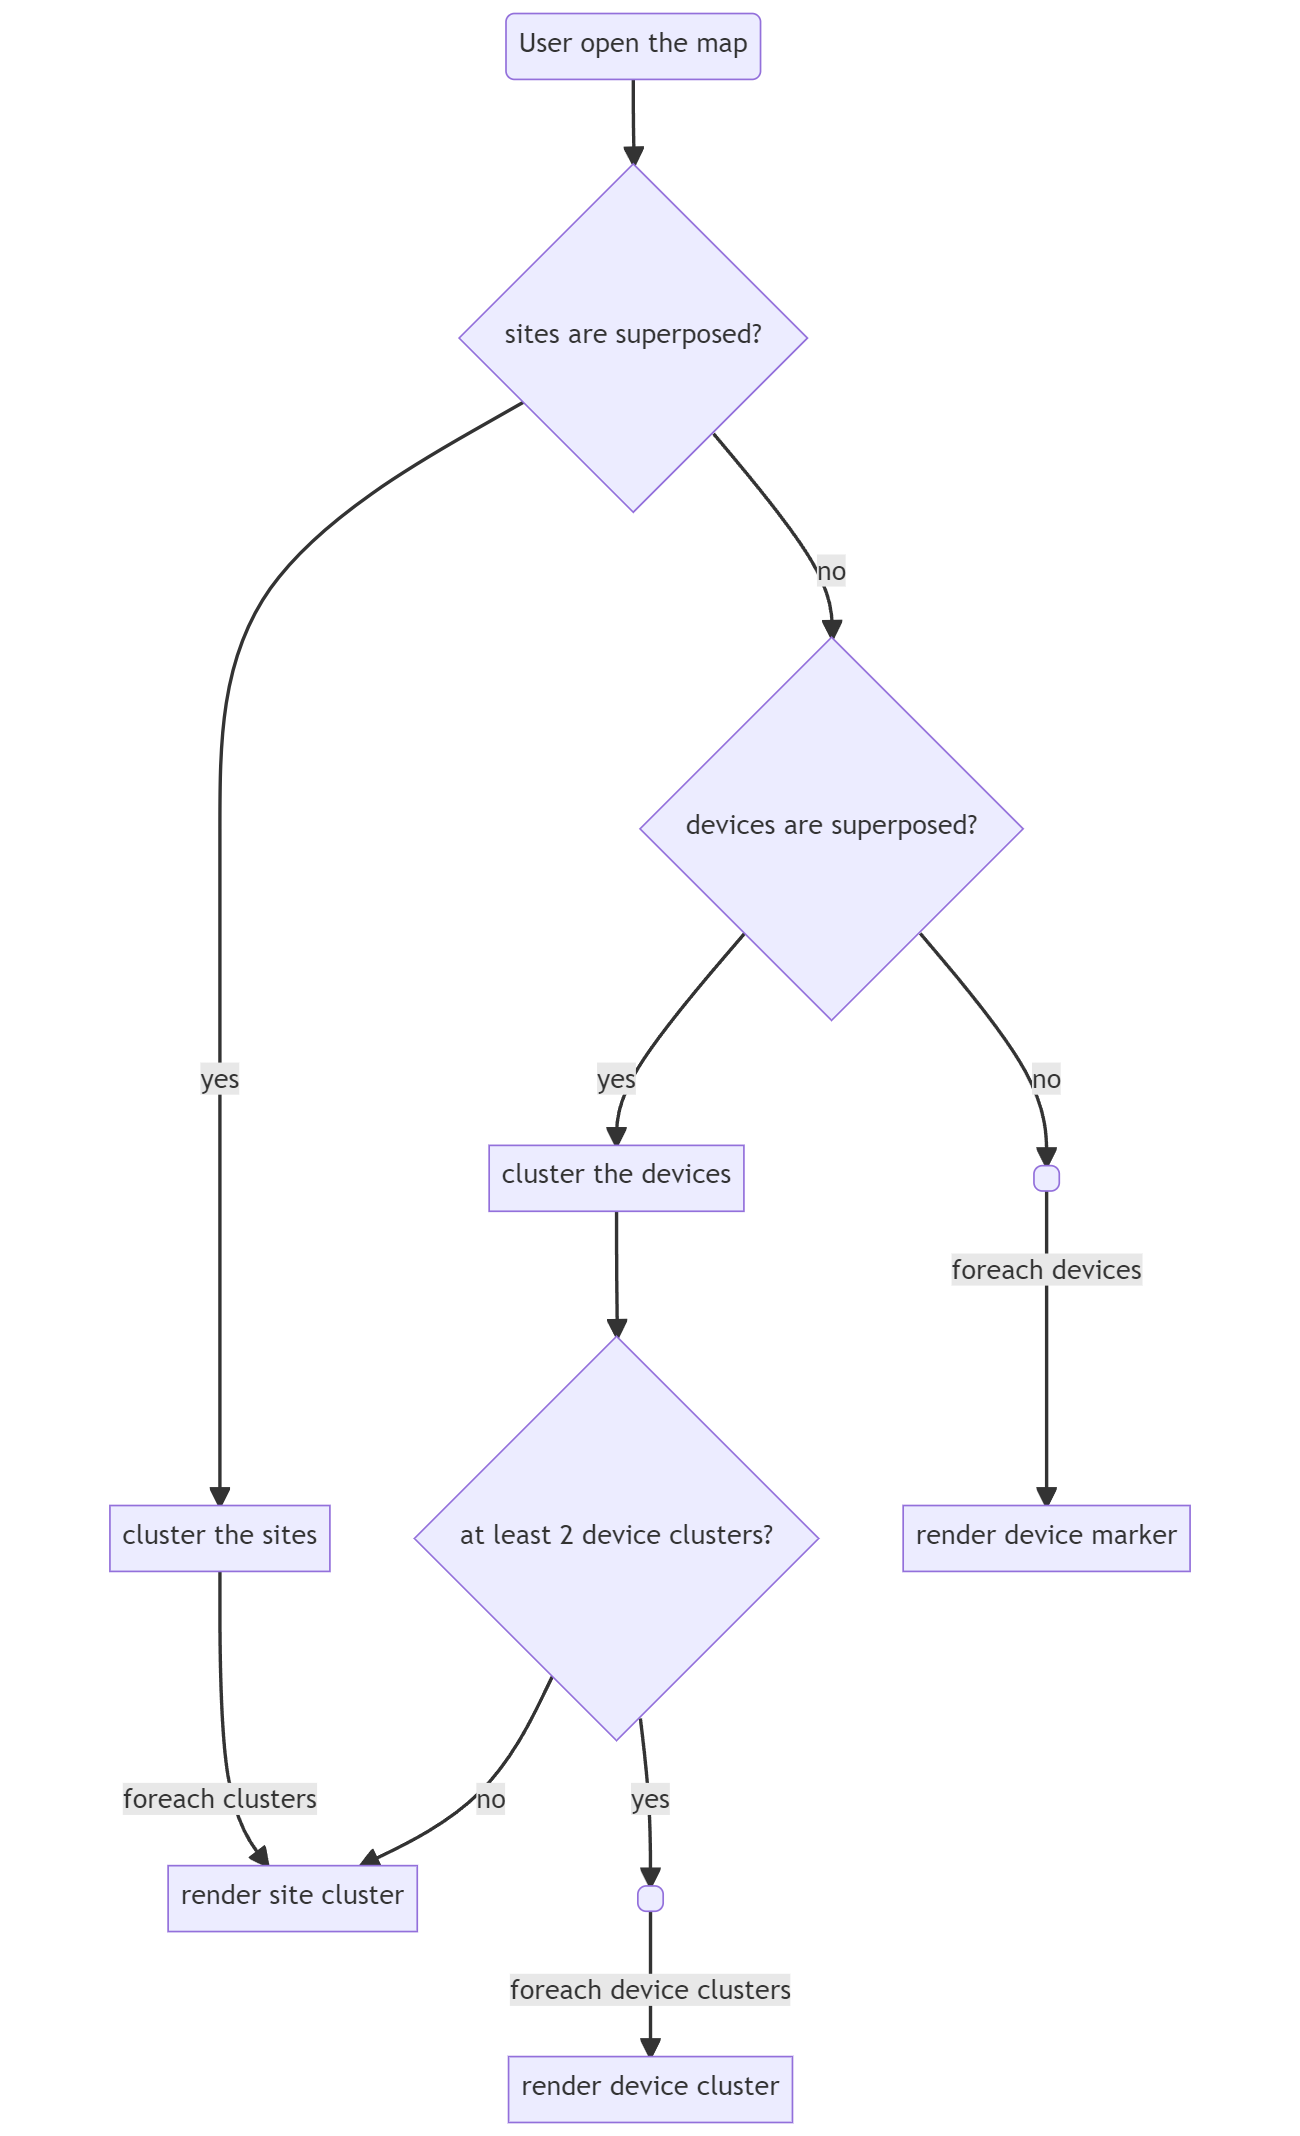
\includegraphics[width=10cm]{map_clustering_flow}
  \caption{Flow-Diagram-Darstellung des zweistufigen Clusterings von \textit{Sites} und Sensoren auf einer interaktiven Karte (Englisch)}
  \label{fig:map_clustering_flow}
\end{figure}

\subsection{Darstellung der Cluster und Marker}

Die aktuelle Karte besteht aus acht verschiedenen Markierungen, die die verschiedenen Arten und den Status der Geräte anzeigen:

\begin{figure}[H]
  \centering
  
\includegraphics[width=10cm]{devices_markers}
  \caption{Marker in Form einer Reißzwecke, die den Standort eines Geräts anzeigen}
  \label{fig:devices_markers}
\end{figure}

Jeweils von links nach rechts stellen sie dar:

\begin{enumerate}
  \item Sensor, der ein Feuer erkennt
  \item Sensor, der offline ist
  \item Sensor mit niedrigem Batteriestand
  \item Sensor, der seine letzte Nachricht vor mehr als 12 Stunden gesendet hat
  \item Sensor, der seine letzte Nachricht vor mehr als 6 Stunden gesendet hat
  \item Aktiver Sensor
  \item Mesh-Gateway
  \item Border-Gateway
\end{enumerate}

Sechs verschiedene Markierungen zu haben, um denselben Gerätetyp anzuzeigen, ist viel zu viel und macht die Verwendung verschiedener Farben weniger relevant.
Es wird empfohlen, eine Palette von maximal fünf Farben zu verwenden \cite{likeChameleon}, damit der Nutzer sie einfach unterscheiden und sich ihre Bedeutung merken kann.
So müssen nur vier Farben verwendet werden, um die verschiedenen Zustände eines Sensors darzustellen.
Dies wird erreicht, indem die Marker 3, 4 und 5 der vorherigen  Liste zu einem einzigen Marker mit der gleichen gelben Farbe wie Marker 5 kombiniert werden.
Dies ist darauf zurückzuführen, dass der Grundstatus hauptsächlich durch eine schlechte Sonneneinstrahlung auf die Solarpaneele oder eine schlechte Abdeckung der LoRa-Verbindung verursacht wurde.
Diese beiden Probleme können direkt vom Kunden behoben werden, indem er einfach einen Sensor neu ausrichtet oder ein Verbindungsrelais hinzufügt.
So wird der neue Status eines Sensors die \textit{Notwendigkeit einer Wartung} anzeigen.\\

Die Karte zeigt nun genau die verschiedenen Geräte eines, aber auch die Position der Cluster von Geräten und \textit{Sites} sowie die Lokalisierung eines einzelnen \textit{Site} müssen dargestellt werden.
In den meisten interaktiven Karten sind Cluster an einem runden Icon zu erkennen, das die Anzahl der enthaltenen Elemente anzeigt und von einem ähnlich gefärbten, aber weniger undurchsichtigen Halo umgeben ist.

\begin{figure}[H]
  \centering
  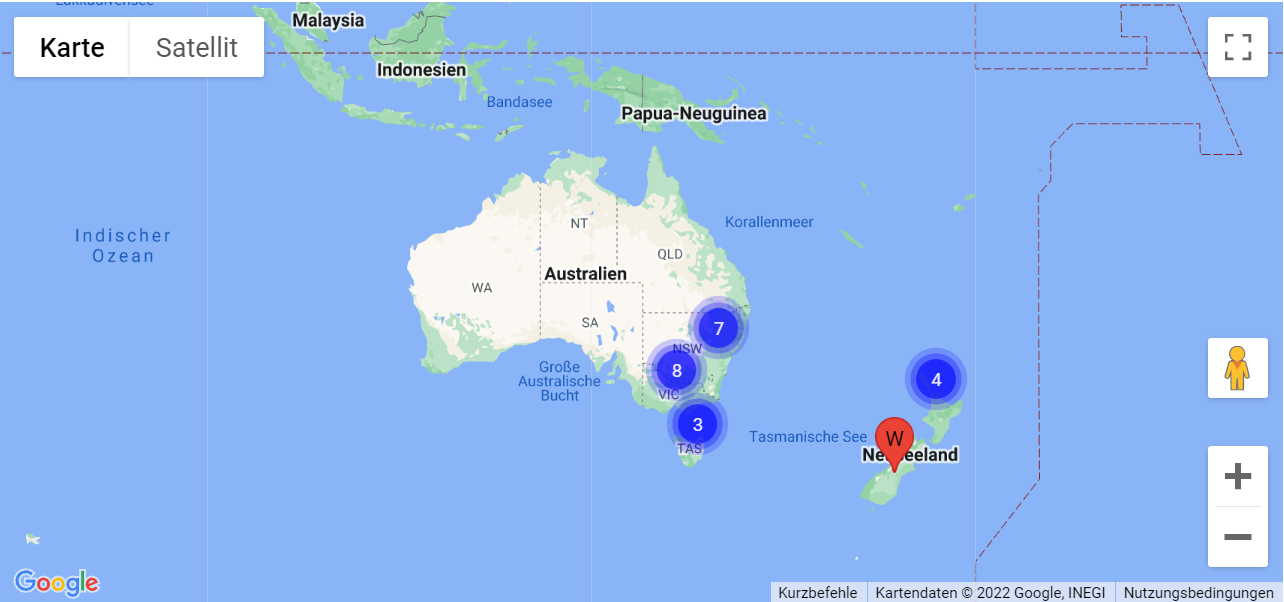
\includegraphics[width=14cm]{google_maps_clusters}
  \caption{Design der Cluster standardmäßig vorhanden auf dem Produkt Google Maps}
  \label{fig:google_maps_clusters}
\end{figure}

Um den Karten von Dryad eine persönliche Note zu verleihen, werden die verschiedenen Cluster durch ein Sechseck dargestellt, das an das Logo des Startups erinnert:

\begin{figure}[H]
  \centering
  
\includegraphics[width=8cm]{clusters_markers}
  \caption{Prototyping von Clustermarkern, die in Version 2 der interaktiven Karten verwendet werden}
  \label{fig:clusters_markers}
\end{figure}

Diese Marker repräsentieren jeweils von links nach rechts:

\begin{enumerate}
  \item Cluster von \textit{Sites}, der einen \textit{Site} enthält, der ein Feuer detektiert
  \item Cluster von \textit{Sites}, der einen \textit{Site} mit einem Offline-Sensor enthält
  \item Cluster von \textit{Sites}, der einen \textit{Site} mit einem wartungsbedürftigen Sensor enthält
  \item Cluster von Standorten
  \item Cluster von Sensoren. Diese Art von Cluster hat die gleichen Farbvariationen wie die \textit{Sites}-Cluster
\end{enumerate}

Die verschiedenen Marker, die Sie verwenden können, sind nun festgelegt.
Um ihr Aussehen entsprechend ihrer Priorität zu verstärken, können Sie die Größe der einzelnen Marker beeinflussen.
So wurde eine Prioritätsskala der Marker und ihrer relativen Größe wie folgt erstellt:

\begin{table}[H]
  \begin{tabular}{p{0.6\linewidth} |p{0.2\linewidth}|p{0.2\linewidth}}
    Markern                                                & Priorität (1: niedrig; 6: hoch) & Relative Größe \\ \hline\hline

    Cluster eines \textit{Site}                            & \textbf{6}                      & x1.11          \\\hline
    Marker einer \textit{Site}                             & \textbf{5}                      & x1             \\\hline
    Cluster von Sensoren in Feuer, offline oder in Wartung & \textbf{4}                      & x0.89          \\\hline
    Cluster von Sensoren                                   & \textbf{2}                      & x0.73          \\\hline
    Marker für einen brennenden Sensor                     & \textbf{4}                      & x0.89          \\\hline
    Marker eines Offline-Sensors                           & \textbf{3}                      & x0.78          \\\hline
    Marker eines Sensors in Wartung                        & \textbf{2}                      & x0.73          \\\hline
    Marker eines Sensors                                   & \textbf{1}                      & x0.55          \\\hline
    Marker eines Border-Gateways                           & \textbf{3}                      & x0.78
  \end{tabular}
  \caption{Festlegung der Prioritäten und Größen der Marker}
\end{table}

Diese relativen Größen bleiben subtil, aber dennoch stark genug, um vom menschlichen Auge erkannt zu werden, wodurch die verschiedenen Prioritäten angezeigt werden können.
Beachten Sie auch, dass eine Markierung mit einer höheren Priorität vor einer Markierung mit einer niedrigeren Priorität angezeigt wird.

\begin{figure}[H]
  \centering
  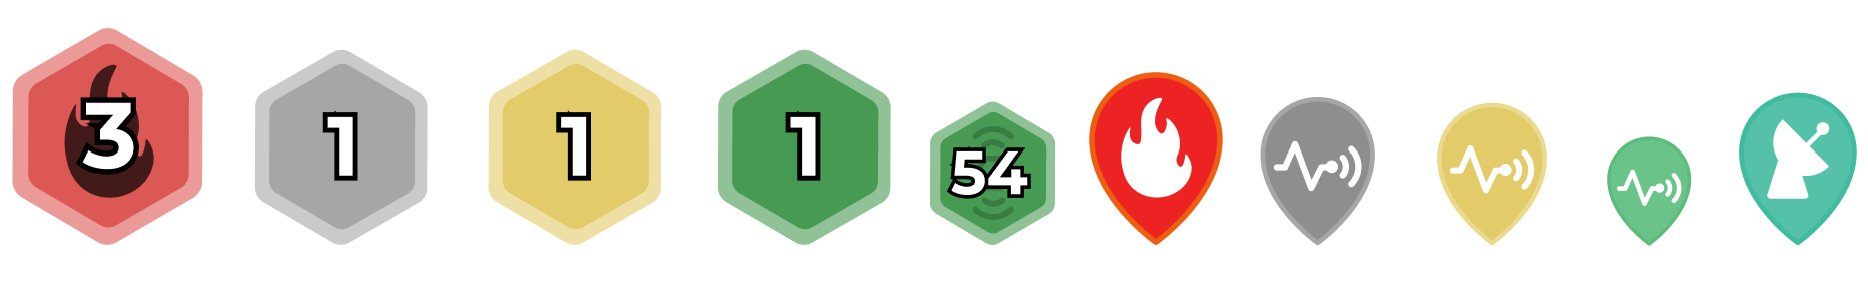
\includegraphics[width=\textwidth]{map_markers_size}
  \caption{Markern mit ihrer relativen Größe auf der Karte}
  \label{fig:map_markers_size}
\end{figure}


\subsection{Hilfe beim Lesen der Karte} \label{sec:help_reading_map}

Die Anzeige verschiedener Markierungen ermöglicht bereits eine gute Erkundung eines Ortes und seiner verschiedenen Sensoren.
Es muss noch sichergestellt werden, dass weitere nützliche Hinweise vorhanden sind, die dem Nutzer das Lesen der Karte erleichtern.
Dies gilt insbesondere für die Darstellung eines Standorts, eines Feuers und auch für Informationen, die in einem Cluster zusammengefasst sind.

Ein Standort wird in Form eines Clustermarkers dargestellt.
Um das Auffinden eines bestimmten \textit{Site} auf einer Karte zu erleichtern, wird der Name des \textit{Site} in einem Popup über dem Marker angezeigt, wenn sich die Maus des Nutzers über dem Marker befindet.

\begin{figure}[H]
  \centering
  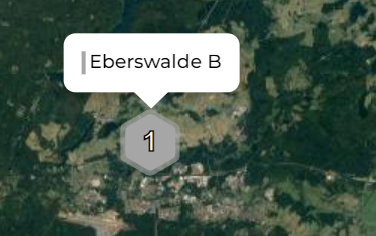
\includegraphics[width=5cm]{map_site_name_window}
  \caption{Popup, das den Namen der \textit{Site} angibt, die von der Maus des Nutzers angehoben wird}
  \label{fig:map_site_name_window}
\end{figure}

Wenn die verschiedenen Geräte einer \textit{Site} in mindestens zwei verschiedenen Clustern angezeigt werden können, verschwindet die Markierung der \textit{Site} und es werden nur noch die Cluster der Geräte angezeigt.
Es ist notwendig, dem Nutzer klar anzuzeigen, zu welcher \textit{Site} diese Geräte gehören.
Um dies zu erreichen, werden die Apparate in einen Bereich eingebettet, der je nach Status der \textit{Site} farbig ist.
Das Popup mit dem Namen der \textit{Site} wird auch sichtbar, wenn der Nutzer mit der Maus über diesen Bereich fährt.

\begin{figure}[H]
  \centering
  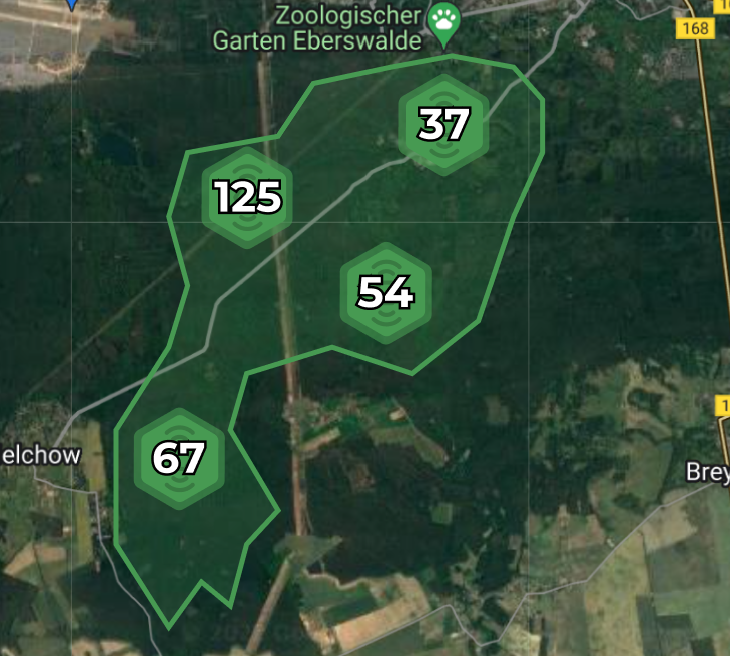
\includegraphics[width=4cm]{map_site_with_zone}
  \caption{Darstellung eines \textit{Site} mit seinem Abdeckungsbereich}
  \label{fig:map_site_with_zone}
\end{figure}

Es ist auch wichtig, jetzt zu definieren, was der Status einer \textit{Site} ist.
Jeder Sensor auf einer \textit{Site} hat einen Status, der Feuer, Offline, Wartung oder Default (nichts zu melden) sein kann.
Ein \textit{Site} oder Sensors-cluster kann Sensoren enthalten, die unterschiedliche Status haben.
Es ist daher notwendig, jedem Status eine Priorität zuzuweisen, um dem Nutzer die relevantesten Informationen anzuzeigen.
So ist es z.B. besser, einen Standort auf der Karte als brennend anzuzeigen, als die Tatsache, dass einer der Sensoren, die ihn bilden, offline ist.

\begin{table}[H]
  \begin{tabular}{p{0.3\linewidth}|p{0.4\linewidth}}
    \centering
    Status     & Priorität (1: niedrig; 4: hoch) \\ \hline\hline

    in Brand   & 4                               \\\hline
    offline    & 3                               \\\hline
    in Wartung & 2                               \\\hline
    Standard   & 1
  \end{tabular}
  \caption{Festlegung der Prioritäten der Status von Sensoren, \textit{Sites} und Clustern}
\end{table}

So hat ein \textit{Site} oder ein Cluster von Sensoren oder ein Cluster von \textit{Sites} den Status (und damit konkret die Farbe) des Sensors mit dem stärksten Status.
Auf diese Weise zeigt ein Cluster nicht alle Informationen der Sensoren an, aus denen er besteht.
Um zu vermeiden, dass der Nutzer die Karte vergrößern muss, um den Status der einzelnen Sensoren zu überprüfen, wird beim Überfahren des Clusters mit der Maus ein Popup mit der Statusverteilung der einzelnen Sensoren eingeblendet.
Diese sollte die Namen der nach Status gruppierten Sensoren sowie einen Balken mit der Verteilung dieser Status anzeigen.

\begin{figure}[H]
  \centering
  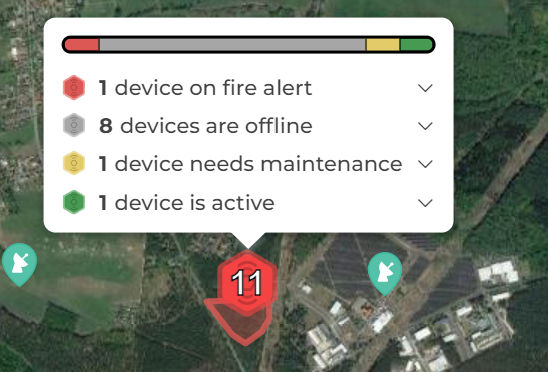
\includegraphics[width=5cm]{map_sensors_window_collapsed}
  \caption{Detailansicht der Sensoren, aus denen ein Cluster besteht}
  \label{fig:map_sensors_window_collapsed}
\end{figure}
\begin{figure}[H]
  \centering
  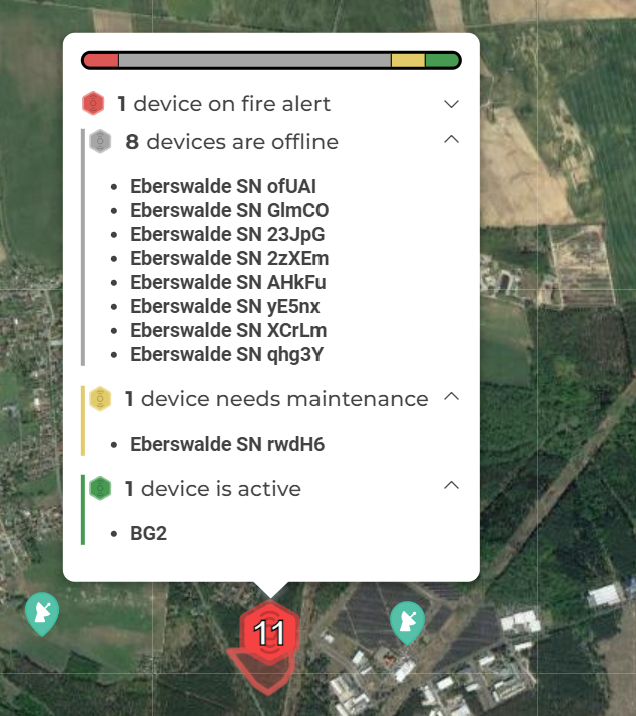
\includegraphics[width=5cm]{map_sensors_window}
  \caption{Detailansicht der Sensoren mit erweiterter Ansicht, die einen Cluster bilden}
  \label{fig:map_sensors_window}
\end{figure}
\begin{figure}[H]
  \centering
  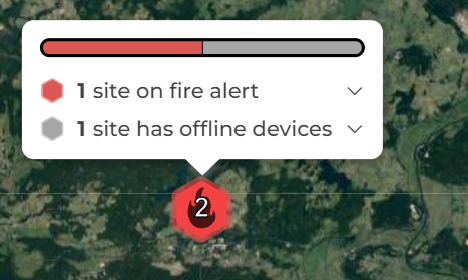
\includegraphics[width=5cm]{map_sites_window}
  \caption{Details zu den \textit{Sites}, aus denen ein Cluster besteht}
  \label{fig:map_sites_window}
\end{figure}

Der stärkste Status ist das Vorhandensein eines Feuers.
Um seine Sichtbarkeit und Erkennung zu verstärken, wird ein Marker eines Sensors mit dem Status \textit{in Feuer} eine Bounce-Animation haben.


\subsection{Interaktion mit der Karte} \label{sec:map_interaction}

Da die Daten nun geografisch gut auf der Karte dargestellt sind, müssen sie interaktiv gestaltet werden, um dem Nutzer das reichhaltigste Erlebnis zu bieten.
In diesem Schritt kann der Nutzer die Karte vergrößern und verkleinern sowie die Ansicht mithilfe von Drag und Drop verschieben.
Dies ermöglicht ihr bereits, die verschiedenen Cluster von Standorten oder Sensoren zu erkunden.
Wenn der Nutzer auf einen Cluster klickt, zoomt die Map bis zu dem Punkt, an dem sich der Cluster in mindestens zwei Einheiten teilt, und zentriert sich auf den Ursprungspunkt des Clusters.
Dasselbe gilt für den Marker eines \textit{Site}: Wenn er angeklickt wird, zoomt die Karte bis zu dem Punkt, an dem mindestens zwei Sensorcluster oder Sensoren auf der Karte sichtbar sind.

Um Details über den gesamten Standort zu erhalten, kann der Nutzer auf den Abdeckungsbereich des Standortes klicken.
Dadurch wird ein Informationsbereich auf der Karte geöffnet.
Ursprünglich war dieser Bereich eine Sprechblase, die neben der Website angezeigt wurde (siehe \ref{fig:map_old_site_details} im Anhang).
Um den UI-Standard der weltweit verbreiteten Anwendung Google Maps zu verwenden und Platz für die Anzeige der Informationen zu sparen, werden die Details in einer verschiebbaren Seitenleiste auf der linken Seite der Karte angezeigt.
Um die ausgewählte \textit{Site} hervorzuheben, wird der Rand des Bereichs vergrößert und gestrichelt dargestellt.

\begin{figure}[H]
  \centering
  \includegraphics[width=\textwidth]{map_site_details}
  \caption{Anzeige eines Details einer \textit{Site} nach Auswahl}
  \label{fig:map_site_details}
\end{figure}

In der gleichen Idee öffnet sich diese Sidebar mit den Details eines Sensors, wenn er ausgewählt ist.
Der Marker des Sensors wird dann von einem kreisförmigen, hellfarbigen Bereich mit einem gestrichelten Rand umgeben.

\begin{figure}[H]
  \centering
  \includegraphics[width=\textwidth]{map_sensor_details}
  \caption{Anzeige eines Details einer Sensor nach Auswahl}
  \label{fig:map_sensor_details}
\end{figure}

\subsection{Zusammenfassung}

Die interaktive Karte und ihr Design wurden mithilfe des Figma-Tools prototypisch erstellt.
Dies ermöglichte es, die neuen Verhaltensweisen und Ziele der Karte mit dem Team zu teilen, bevor mit der Implementierung begonnen wurde.
Das vorgestellte Design basiert auf einer Version des Verhaltens der Karte, die vom Cloud-Team, der UI-Designerin und sogar dem \ac{CTO} des Unternehmens genehmigt wurde.
Screenshots des Prototyps des Zoomverhaltens der Karte finden Sie im Anhang zum Abschnitt \ref{appendix:map_flow}.
